\documentclass[a4paper,12pt]{article}

\usepackage{hyperref}
\usepackage{cmsrb}
\usepackage[T1]{fontenc}
\usepackage[serbian]{babel}
\usepackage[utf8]{inputenc}
\usepackage{csquotes}
\usepackage{lmodern}
\usepackage{graphicx}
\usepackage{caption}
\usepackage[
	backend=biber,
	style=alphabetic,
	sorting=ynt
]{biblatex}
\addbibresource{citation.bib}
\usepackage{amsmath}
\usepackage{amsfonts}
\usepackage{float}
\usepackage{todonotes}

\hypersetup{
	colorlinks,
	citecolor=black,
	filecolor=black,
	linkcolor=blue,
	urlcolor=blue
}

\renewcommand{\contentsname}{Sadržaj}

\title{Automatsko prepoznavanje teksta sa tablica \todo[color=green!40]{vozila, ne nuzno automobila?}automobila koristeći Jedinstveni Vizuelni Model za Prepoznavanje Teksta na Sceni}
\date{}

\begin{document}
	\emergencystretch 3em
	\begin{titlepage}
		\pagenumbering{gobble} % Remove page numbering
		\centering
		{\huge\bfseries \maketitle}
		
		{\large
			\textbf{Student:}
			Andrija Urošević
			\par
			\bigskip
			\textbf{Mentor:}
			dr Nemanja Ilić
		}
	
		\vfill
		{\large Računarski fakultet,\par}
		{\large Univerzitet Union\par}
		\bigskip
		\date{Septembar 2024}
	\end{titlepage}
	
	\pagenumbering{roman}
	
	\section*{Predgovor}
	\addcontentsline{toc}{section}{Predgovor}
	\noindent
	\todo[color=green!40]{Prostor za predgovor.}
	\newpage
	
	\tableofcontents
	\newpage
	
	\pagenumbering{arabic}
	
	\section*{Sažetak}
	\addcontentsline{toc}{section}{Sažetak}
	\noindent
	Automatsko prepoznavanje teksta sa registarskih tablica automobila od izuzetne je važnositi za savremene sisteme nadzora saobraćaja, praćenje vozila i obezbeđenje sigurnosti na putevima. Identifikacija registarskih tablica ima različite primene, uključujući praćenje ukradenih vozila, naplatu putarine, sigurnosne provere i nadzor saobraćaja. U proteklim decenijama, napredak u oblasti obrade slike i mašinskog učenja omogućio je razvoj efikasnih sistema za automatsko prepoznavanje teksta sa tablica vozila. Primena dubokih neuronskih mreža i algoritama dubokog učenja omogućila je visoku tačnost prepoznavanja teksta, čak i u složenim scenama i različitim uslovima snimanja. Ovaj rad istražuje metode i tehnike za automatsko prepoznavanje teksta sa tablica automobila, sa ciljem razvoja sistema koji može precizno identifikovati registarske tablice u realnom vremenu. Eksperimentalni rezultati prikazuju performanse sistema u stvarnim uslovima i ukazuju na mogućnosti za primenu u različitim oblastima, uključujući nadzor saobraćaja, bezbednosne provere i identifikaciju vozila.
	\newpage
	
	\section*{Rečnik stručnih pojmova}
	\addcontentsline{toc}{section}{Rečnik stručnih pojmova}
	\noindent
	\begin{tabular}{l@{\hspace{40pt}}l}
		\textbf{Overfitting} & \textit{Prekomerna prilagođenost} \\
		\textbf{Batch} & \textit{Grupa podataka} \\
		\textbf{Learning rate} & \textit{Stopa učenja} \\
		\textbf{Base model} & \textit{Inicijalni model} \\
	\end{tabular}
	\newpage
	
	\section{Uvod}
	Automatsko prepoznavanje teksta je ključna tehnologija u oblasti kompjuterske vizije koja ima široku primenu u različitim aplikacijama, uključujući prepoznavanje registarskih tablica vozila, prepoznavanje rukopisa, prepoznavanje dokumenata i mnoge druge. Glavni cilj automatskog prepoznavanja teksta je pretvaranje vizuelno prikazanog teksta u format koji računari mogu razumeti i obrađivati, omogućavajući im da interpretiraju tekstualne informacije slično kao što to radi čovek.
		
	Automatsko prepoznavanje teksta sa registarskih tablica automobila obuhvata nekoliko ključnih koraka koji se odvijaju u procesu od prikupljanja podataka do konačne integracije sistema u softver za prepoznavanje tablica automobila.
	
	Prikupljanje raznovrsnog skupa slika registarskih tablica vozila ključno je za uspešno treniranje modela. Ove slike treba da obuhvataju različite tipove tablica, različite uslove osvetljenja i pozadine kako bi model bio što robustniji. Nakon prikupljanja, slike treba pažljivo razvrstati na one koje su pogodne za treniranje modela i one koje nisu. Ovo uključuje filtriranje slika sa veoma lošim kvalitetom, zamućenim ili nejasnim tablicama. Kako bi se obogatio skup podataka i poboljšala generalizacija modela, potrebno je primeniti tehnike augmentacije podataka. Ovo uključuje manipulaciju sa slikama kao što su rotacija, promena osvetljenja, izobličenja i dodavanje šuma. Pored toga, sintetički podaci se mogu generisati korišćenjem programa za generisanje tablica sa tekstom. Svaka slika mora biti precizno označena sa tačnim tekstualnim sadržajem registarske tablice kako bi se koristila za obuku modela. Ovaj proces može biti ručan ili se može koristiti alat za automatsko lejbelovanje. Nakon pripreme podataka, sledi faza treniranja mreže za prepoznavanje teksta. U ovoj fazi, model se obučava nad označenim podacima kako bi naučio da prepoznaje tekst sa slika tablica. Kada je model obučen, integriše se u softver za prepoznavanje tablica automobila. Ovaj softver obično obuhvata module za detekciju tablica, detekciju teksta na tablicama, formatiranje izlaza i druge funkcionalnosti.
	
	Kako bi omogućili portabilnost i lakšu distribuciju sistema za prepoznavanje tablica, koristi se Docker kontejner. Docker omogućava pakovanje softverskih aplikacija i njihovo pokretanje u izolovanim okruženjima. Još jedna od bitnih komponenata je Python web framework - FastAPI koji omogućava brzo kreiranje API-ja za komunikaciju sa softverskim komponentama. Integracija Docker-a i FastAPI modula omogućava da se servis za prepoznavanje teksta koristi nezavisno od platforme na kojoj se izvršava, čineći ga pristupačnim i jednostavnim za upotrebu u različitim okruženjima.
	\newpage
	
	\section{Prepoznavanje teksta}
	\subsection{Uvod u prepoznavanje teksta}
	Prepoznavanje teksta na sceni ima za cilj da tekst sa slika konvertuje u digitalni niz karaktera, što prenosi semantiku visokog nivoa ključnu za razumevanje scene. Zadatak prepoznavanja teksta sa scene je izazovan zbog varijacija u: deformacijama teksta, fontovima, preklapanjima različitih tekstova, prekompleksnim pozadinama, itd. Dodatno, otežavajući faktor može biti i to što se tekst može pojaviti pod različitim uglovima.
	
	\begin{figure}[H]
		\centering
		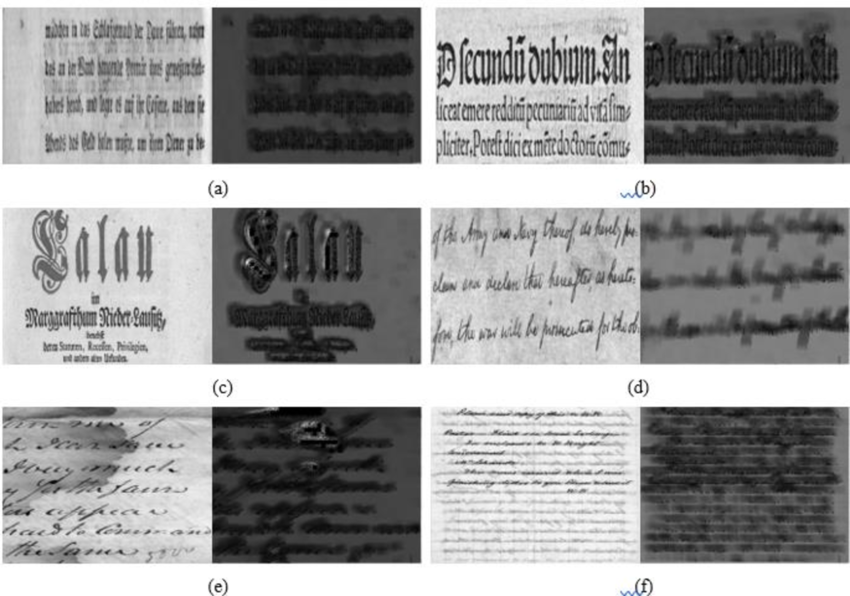
\includegraphics[width=\textwidth]{assets/text.png}
		\caption{Tekst na sceni sa različitim fontovima, pozadinama, osvetljenjem i slično}
		\label{fig:text-on-scene}
	\end{figure}
	
	U proteklim godinama uloženi su brojni napori kako bi se poboljšala tačnost prepoznavanja teksta. Moderni pristupi za prepoznavanje teksta, pored tačnosti, takođe uzimaju u obzir i faktore poput brzine izvršavanja modela zbog praktičnih zahteva.
	
	Metodološki, prepoznavanje teksta na sceni može se posmatrati kao prelazak iz modaliteta slike u niz karaktera. Obično, prepoznavanje teksta se sastoji od dva osnovna dela, vizuelnog modela za ekstrakciju karakteristika i sekvencijskog modela za transkripciju teksta.
	\newpage
	
	\subsection{Istorijski pregled prepoznavanja teksta}
	
	Prvi primeri i prva faza tehnologije optičkog prepoznavanja karaktera(OCR) pojavili su se sredinom 20. veka, pretežno tokom 1950-ih i 1960-ih godina. Ovo doba obeležilo je razvoj ranih sistema OCR-a, koji su koristili osnovne tehnike prepoznavanja obrazaca kako bi prepoznali mašinski odštampane karaktere. Ovi sistemi su često bili ograničeni na prepoznavanje određenih fontova i imali su relativno nisku stopu tačnosti u poređenju sa modernom OCR tehnologijom. Glavna primena im je bila čitanje standardizovanih obrazaca i dokumenata sa jasno štampanim tekstom i poznatim fontom.
	
	Druga faza tehnologije optičkog prepoznavanja karaktera dogodila se krajem 20. veka i početkom 21. veka, počevši oko 1970-ih i nastavljajući se u 2000-ima. Ovo doba je obeleženo značajnim napretkom u tehnologiji OCR-a, uključujući razvoj sofisticiranih algoritama i tehnika za prepoznavanje karaktera. Ovi napredci doveli su do veće tačnosti i mogućnosti prepoznavanja šireg spektra fontova, jezika i rasporeda dokumenata. Dodatno, integracija pristupa mašinskog učenja i neuronskih mreža doprinela je daljem poboljšanju performansi OCR-a. U ovoj fazi došlo je do primene OCR sistema u širem spektru aplikacija, od skeniranja i konverzije dokumenata u digitalno arhiviranje, do automatizovanog unosa podataka i ekstrakcije teksta u različitim industrijama.
	
	Treća faza tehnologije optičkog prepoznavanja karaktera je trenutno aktuelna i predstavlja trenutno stanje napretka u sistemima OCR-a. Ovo doba karakteriše integracija najnovijih tehnologija poput dubokog učenja, konvolucionih neuronskih mreža (CNN) i rekurentnih neuronskih mreža (RNN) u algoritme OCR-a. Ove napredne tehnike značajno su poboljšale tačnost i pouzdanost sistema OCR-a, omogućavajući prepoznavanje složenih dokumenata sa različitim fontovima, rasporedima i jezicima. Osim toga, pojava OCR usluga zasnovanih na cloud-u i integracija OCR funkcionalnosti u mobilne uređaje učinili su OCR dostupnijim i svestranijim nego ikad ranije. Treća faza takođe obuhvata napretke u analizi i razumevanju dokumenata, omogućavajući OCR sistemima da izvlače ne samo tekst već i strukturalne i semantičke informacije iz dokumenata, što dovodi do poboljšanih sposobnosti obrade dokumenata i pretraživanja informacija.
	
	\subsection{Arhitekture modela za prpoznavanje teksta na slici}
	
	\begin{figure}[H]
		\centering
		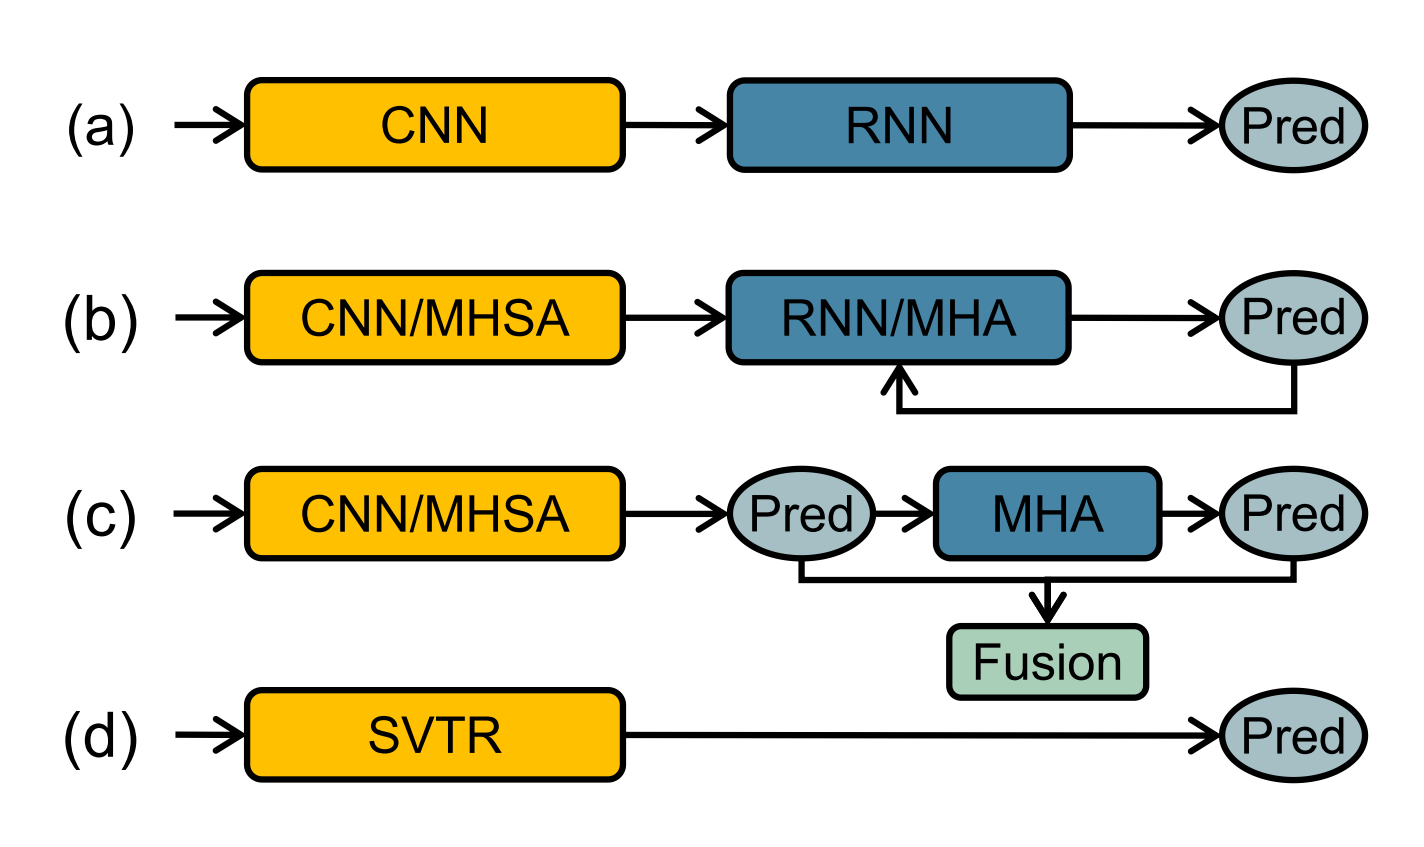
\includegraphics[width=\textwidth]{assets/text-recognition-model-architectures.png}
		\caption{Arhitekture modela za prepoznavanje teksta sa scene. (a) Modeli zasnovani na CNN-RNN. (b) Modeli kodiranja-dekodiranja. (c) Vizuelno-jezički modeli. (d) SVTR, koji prepoznaje tekst scene sa jedinstvenim vizuelnim modelom i odlikuje se efikasnošću, tačnošću i višejezičnom svestranošću.}
		\label{fig:tr-model-architectures}
	\end{figure}
	
	Modeli zasnovani na CNN-RNN \cite{shi2015endtoend} prvo koriste CNN za ekstrakciju karakteristika. Karakteristike se zatim preoblikuju u sekvencu koju BiLSTM modeluje uz pomoć CTC gubitka kako bi generisao predikciju (Slika \ref{fig:tr-model-architectures}(a)). Odlikuju se efikasnošću i ostaju izbor za neke komercijalne proizvode za prepoznavanje teksta sa scene. Međutim, preoblikovanje karakteristika u sekvencu je osetljivo na deformacije teksta, što ograničava efikasnost takvih modela.
	
	Kasnije su pristupi zasnovani na auto-regresivnim metodama kodera-dekodera postale popularne \cite{sheng2019nrtr, li2019show, zheng2023cdistnet}. Ove metode transformišu prepoznavanje u iterativni proces dekodiranja (Slika \ref{fig:tr-model-architectures}(b)). Kao rezultat, postignuta je poboljšana tačnost jer je uzeta u obzir kontekstualna informacija. Međutim, brzina izvođenja je spora zbog transkripcije karakter po karakter. Ovaj postupak je dodatno proširen na softversku strukturu zasnovanu na viziji i jeziku \cite{yu2020accuratescenetextrecognition, fang2021readlikehumansautonomous}, gde je jezičko znanje uključeno (Slika \ref{fig:tr-model-architectures}(c)) i sprovedena je paralelna predikcija. Ipak, ovaj postupak često zahteva model sa velikim kapacitetom ili složenu paradigmu prepoznavanja kako bi se osigurala tačnost prepoznavanja, što ograničava njegovu efikasnost.
	
	U poslednje vreme, naglasak je na razvoju pojednostavljenih arhitektura kako bi se dobilo na brzini izvršavanja. Na primer, korišćenje složene paradigme obuke, ali jednostavnog modela za izvršavanje. Rešenje zasnovano na CRNN-RNN ponovo je pregledano u sledećem radu: \cite{Hu_Cai_Hou_Yi_Lin_2020}. Koristi mehanizam pažnje i grafovsku neuronsku mrežu za agregaciju sekvencijalnih karakteristika koje odgovaraju istom karakteru. Pri izvršavanju, deo za modelovanje zasnovan na mehanizmu pažnje je odbačen kako bi se uskladila tačnost i brzina.
	
	Nedavni uspeh transformera za obradu slike \cite{dosovitskiy2021imageworth16x16words, liu2021swintransformerhierarchicalvision}, inspirisao je nastanak jedinstvenog vizuelnog modela za prepoznavanje teskta na sceni(SVTR) \cite{du2022svtrscenetextrecognition}. SVTR najpre razlaže tekst slike na male 2D isečke koji se nazvaju komponente karaktera, od kojih svaka komponenta može sadržati samo deo karaktera. Tokenizacija slike po isečcima praćena mehanizmom samopažnje se primenjuje da bi se uhvatile indicije prepoznavanja teksta među komponentama karaktera. Za ovu svrhu je razvijena prilagođena arhitektura za tekst, čija osnovna struktura sadrži progresivno smanjujuću visinu mape karakteristika u tri faze i uključujue operacije mešanja, spajanja i/ili kombinovanja. Osmišljeni su lokalni i globalni blokovi mešanja koji se rekurzivno primenjuju u svakoj fazi, zajedno sa operacijom spajanja ili kombinovanja, stičući tako afinitete na nivou lokalnih komponenti koje predstavljaju karakteristike slične potezima karaktera i dugoročne zavisnosti između različitih karaktera. Dakle, osnovna struktura ekstraktuje karakteristike komponenti na različitim rastojanjima i na više skala, formirajući višeslojnu percepciju karakteristika karaktera. Kao rezultat, prepoznavanje teksta se postiže jednostavnom linearnom predikcijom. U celom procesu koristi se samo jedan vizuelni model (Slika \ref{fig:tr-model-architectures}(d)).

	\subsection{Korišćenje Jedinstvenog Vizuelnog Modela za Prepoznavanje Teksta na Sceni}
	
	Tradicionalni modeli za prepoznavanje teksta obično uključuju dve odvojene komponente: vizuelni model za izdvajanje karakteristika sa slike i sekvencijalni model za dekodiranje izdvojenih karakteristika u tekst. Jedinstveni vizuelni model za prepoznavanje teksta na sceni(SVTR) eliminiše potrebu za sekvencijalnim modelom u potpunosti, čineći ga jednostavnijim i efikasnijim.
	
	Uklanjanjem komponente sekvencijalnog modeliranja, SVTR postiže konkurentnu preciznost na zadacima prepoznavanja teksta, pružajući veću efikasnost u poređenju sa tradicionalnim metodama.
	
	\subsubsection{Arhiterktura}

	Pregled SVTR modela je prikazan na (Slika \ref{fig:svtr-architecture}) i predstavlja tro-faznu mrežu sa progresivno smanjujućom visinom, namenjenu za prepoznavanje teksta. Slika teksta veličine H×W×3, prvo se transformiše u \(\dfrac{H}{4} \times \dfrac{W}{4}\) isečaka dimenzije \(D_0\) koristeći progresivno preklapajuće ugrađivanje isečaka. Isečci predstavljaju karakterne(znakovne) komponente, od kojih svaka odgovara delu tekstualnog karaktera na slici. Zatim se izvode tri faze, od kojih se svaka sastoji od niza blokova za mešanje praćenih operacijom spajanja ili kombinovanja, na različitim skalama za ekstrakciju karakteristika. Osmišljeni su lokalni i globalni blokovi za mešanje za ekstrakciju lokalnih obrazaca nalik potezima i hvatanje međukomponentne zavisnosti. Pomoću osnovne strukture se karakterizuju komponentne karakteristike i zavisnosti na različitim udaljenostima i na više skala, predstavljene kao C veličine \(1 \times \dfrac{W}{4} \times D_3\), koje percipira karakteristike znakova na više nivoa granularnosti. Na kraju procesa, model istovremeno predviđa sve znakove sa ulazne slike i primenjuje postupak uklanjanja duplikata kako bi se eliminisali eventualno pogrešno ponovljeni karakteri koje je model predvideo, a koji nisu stvarno prisutni na originalnoj slici. Rezultat ovog procesa je konačan niz prepoznatih znakova.

	\begin{figure}[H]
		\centering
		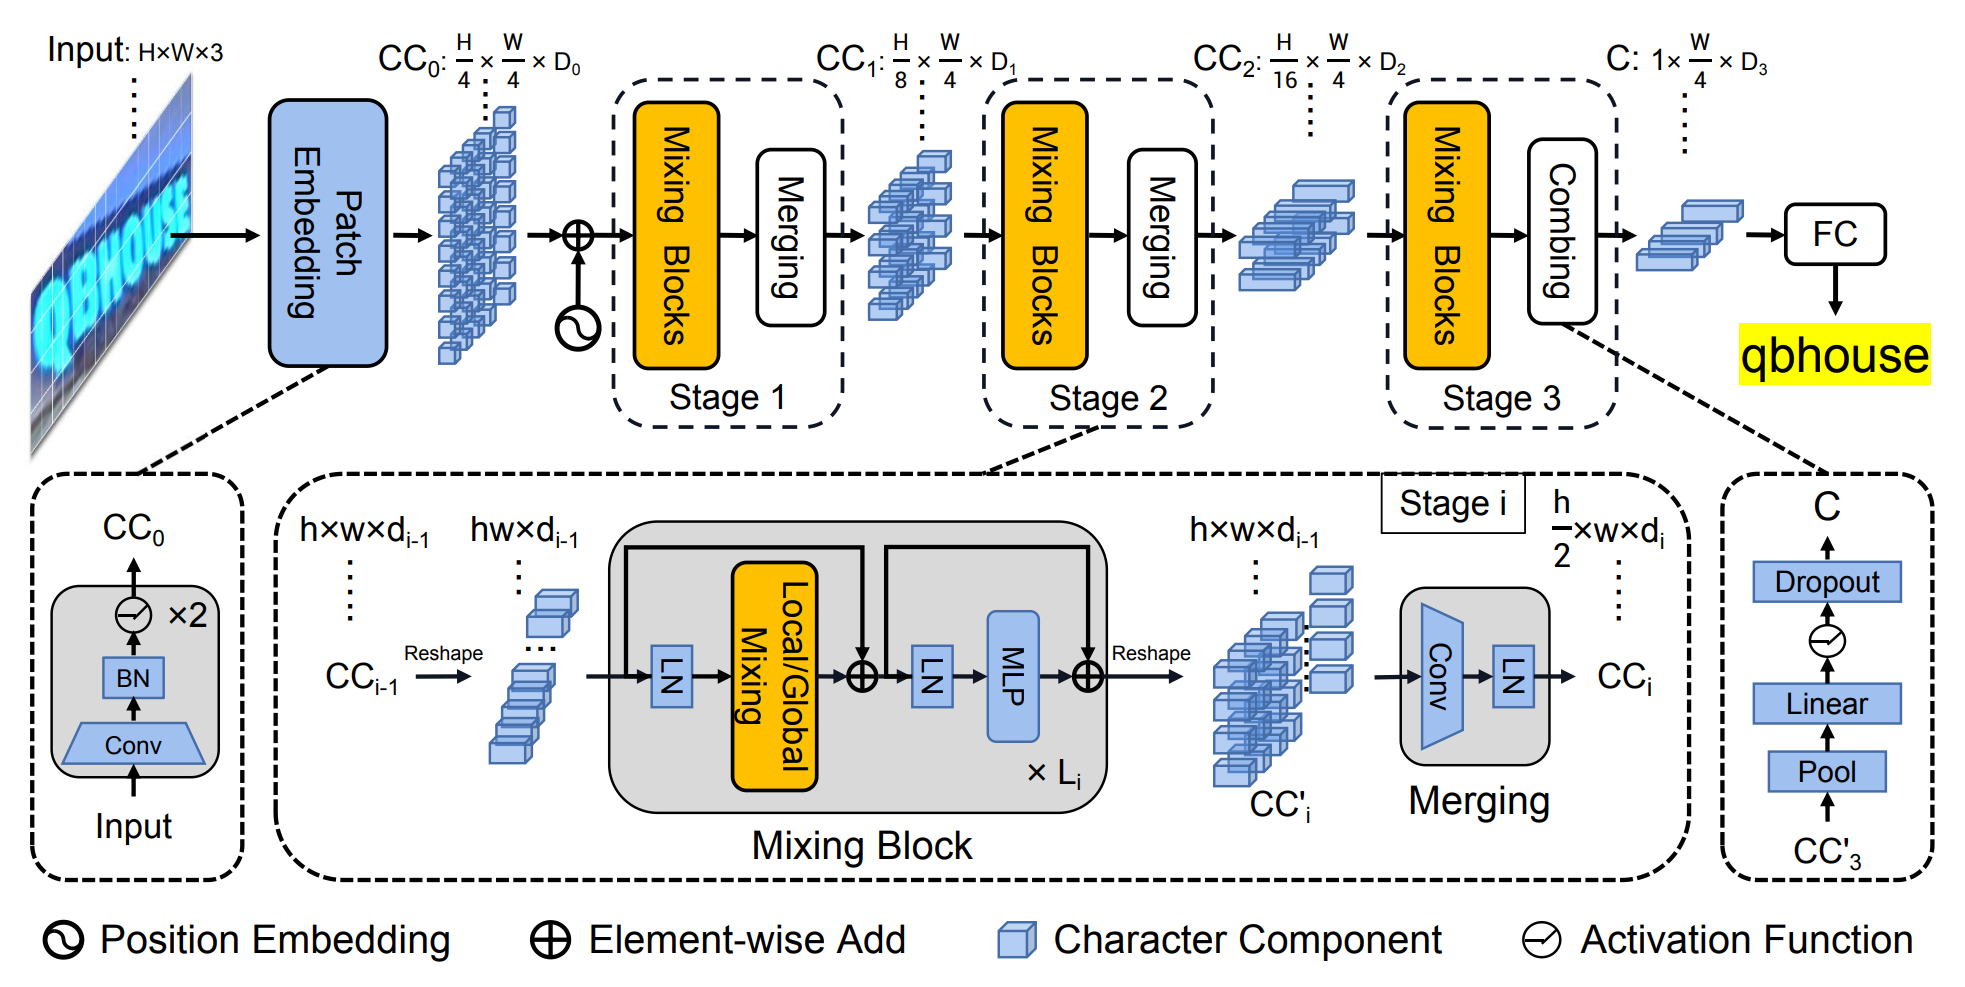
\includegraphics[width=\textwidth]{assets/svtr-architecture.png}
		\caption{Arhitektura SVTR-a: Mreža koja kroz tri faze progresivno smanjuje visinu mape karakteristika. U svakoj fazi se izvodi niz blokova za mešanje, nakon čega sledi operacija spajanja ili kombinovanja. Na kraju se prepoznavanje vrši linearnim predviđanjem.}
		\label{fig:svtr-architecture}
	\end{figure}
	
	\subsubsection{Progresivno preklapajuće ugrađivanje isečaka}
	
	Pvri korak u obradi slike teksta je njeno razlaganje na manje delove koje nazivamo isečcima. Dobijanje karakterističnih isečaka koji predstavljaju komponente znakova znači prelazak iz \(X \in \mathbb{R}^{H \times W \times D_0}\) u \(CC_0 \in \mathbb{R}^{\dfrac{H}{4} \times \dfrac{W}{4} \times D_0}\). Postoje dva uobičajena načina da se ovo uradi — korišćenje \(4 \times 4\) mreže za podelu slike i linearna transformacija svakog dela(Slika \ref{fig:linear-projection-in-ViT}(a)) i korišćenje \(7 \times 7\) konvolucionog filtera sa korakom 4. Autori SVTRa su izabrali alternativni metod. Oni koriste dva manja konvoluciona filtera \(3 \times 3\) jedan za drugim sa korakom 2, kao što je prikazano na (Slika \ref{fig:linear-projection-in-ViT}(b)). Takođe koriste tehniku zvanu normalizacija serije da bi održali brojeve pod kontrolom. Ovaj novi metod zahteva nešto više računarske snage, ali je bolji u kombinovanju karakteristika iz slike.

	\begin{figure}[H]
		\centering
		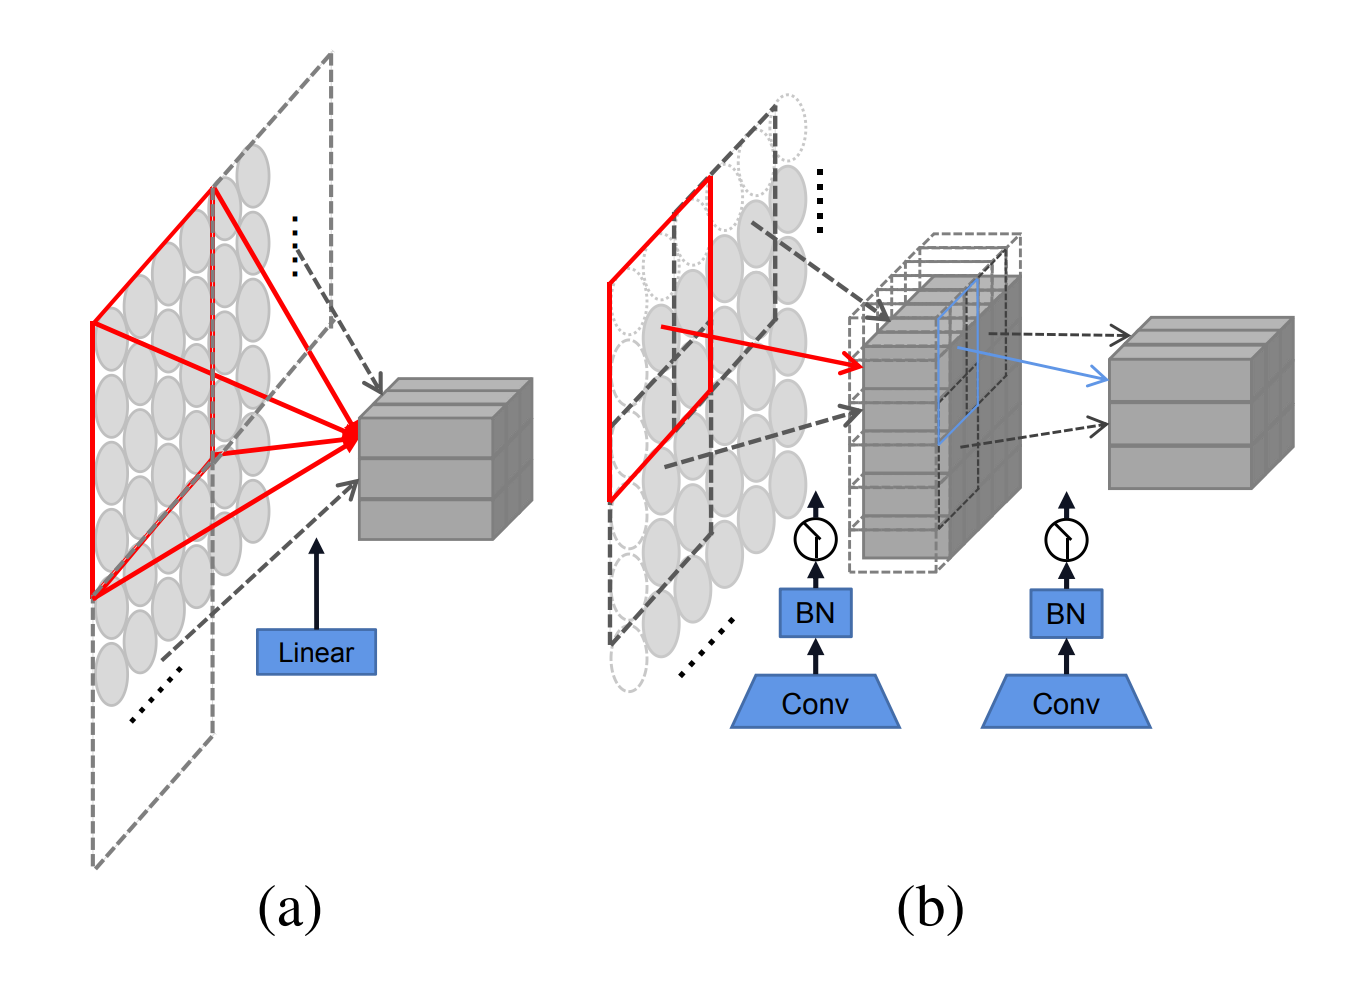
\includegraphics[width=\textwidth]{assets/linear-projection-in-ViT.png}
		\caption{(a) Linearna projekcija u ViT \cite{dosovitskiy2021imageworth16x16words}. (b) SVTR progresivno preklapajuće ugrađivanje isečaka.}
		\label{fig:linear-projection-in-ViT}
	\end{figure}
	
	\subsubsection{Blok \todo[color=green!40]{pronađi prikladniji termin od 'mešanje'}mešanja}
	S obzirom na to da se dva karaktera mogu blago razlikovati važno je posmatrati male delove koji čine karaktere. Prepoznavanje teksta se u velikoj meri oslanja na ekstrakciji karakteristika na nivou komponenti karaktera. Međutim, postojeće studije uglavnom koriste niz karakteristika za predstavljanje teksta na slici. Svaka karakteristika odgovara deliću regiona slike, koji je često nerazumljiv, posebno za nepravilan tekst — što nije optimalno za opisivanje karaktera. Nedavni napredak u vizuelnim transformatorima uvodi 2D reprezentaciju karakteristika, ali njeno korišćenje u kontekstu prepoznavanja teksta je još uvek u fazi istraživanja. Autori SVTRa sugerišu da su dve vrste karakteristika važne za prepoznavanje teksta. Prva su lokalni obrasci, kao što su mali detalji koji čine karakter, poput poteza. Oni pokazuju kako su različiti delovi karaktera međusobno povezani i stvaraju se morfološke karakteristike i korelacije između različitih delova karaktera. Druga su međukarakterne zavisnosti, koje se odnose na to kako su različiti karakteri povezani jedni s drugima, ili kako se tekst odnosi na netekstualne delove slike. Da bi uhvatili ove karakteristike, autori su kreirali dva posebna bloka mešanja. Ovi blokovi koriste tehniku zvanu samopažnja, koja pomaže modelu da se fokusira na važne delove slike. Koristeći dva različita područja fokusa koja mehanizam samopažnje razmatra, ovi blokovi mogu uhvatiti i male detalje i širu sliku o tome kako su karakteri međusobno povezani.
	
	\paragraph{Globalno mešanje}
	Kao što se vidi na (Slici \ref{fig:linear-projection-in-ViT}(a)), globalno mešanje procenjuje zavisnost među svim komponentama karaktera. S obzirom da su tekstualni i ne-tekstualni sadržaj dva glavna elementa na slici, takvo generalno mešanje može uspostaviti dugoročnu zavisnost među komponentama različitih karaktera. Pored toga, ono je takođe sposobno da oslabi uticaj ne-tekstualnih komponenti, istovremeno pojačavajući važnost tekstualnih komponenti. Matematički, za komponente karaktera \(CC_{i-1}\) iz prethodne faze, prvo se vrši njihovo preoblikovanje u niz karakteristika. Pri uvođenju u blok mešanja, primenjuje se normalizacija sloja, a zatim se koristi multi-head samopažnja za modelovanje zavisnosti. Nakon toga, sekvencijalno se primenjuju normalizacija sloja i MLP za fuziju karakteristika.  Zajedno sa prečicama, formira se blok globalnog mešanja.
	
	\paragraph{Lokalno mešanje}
	Kao što se vidi na (Slici \ref{fig:linear-projection-in-ViT}(b)), lokalno mešanje procenjuje korelaciju među komponentama unutar unapred definisanog prozora. Njegov cilj je da kodira morfološke karakteristike karaktera i uspostavi veze između komponenti unutar jednog karaktera, što simulira karakteristiku nalik potezu koja je vitalna za identifikaciju karaktera. Za razliku od globalnog mešanja, lokalno mešanje razmatra okolinu za svaku komponentu. Slično konvoluciji, mešanje se odvija koristeći pristup klizećeg prozora. Veličina prozora je empirijski postavljena na \(7 \times 11\). U poređenju sa globalnim mešanjem, lokalno implementira mehanizam samopažnje za detekciju lokalnih obrazaca. Kao što je prethodno pomenuto, dva bloka mešanja imaju za cilj izvlačenje različitih karakteristika koje su komplementarne. U SVTR-u, blokovi se rekurentno primenjuju više puta u svakoj fazi za sveobuhvatnu ekstrakciju karakteristika.
	
	\subsubsection{Spajanje}
	Održavanje konstantne prostorne rezolucije kroz faze je računski skupo, što takođe dovodi i do redudantnosti reprezentacije karakteristika kroz slojeve. Kao posledica toga, autori SVTR-a osmišljavaju operaciju spajanja nakon blokova mešanja u svakoj fazi (osim u poslednjoj). Karakteristikama koje su izlaz iz poslednjeg bloka mešanja, se prvo menja dimenzija u veličinu \(h \times w \times d_{i-1}\), gde h, w i \(d_{i-1}\) označavaju trenutnu visinu, širinu i broj kanala, redom. Zatim se primenjuje konvolucija veličine \(3 \times 3\) sa korakom 2 u dimenziji visine i korakom 1 u dimenziji širine, praćenu normalizacijom sloja, generišući novi sloj dimenzije \(\dfrac{h}{2} \times w \times d_i\).
	
	Operacija spajanja prepolovljava visinu dok zadržava konstantnu širinu. Ovo ne samo da smanjuje vremenske troškove obrade, već takođe gradi hijerarhijsku strukturu prilagođenu tekstu. Tipično, većina tekstova na slikama se pojavljuje horizontalno ili blizu horizontalno. Kompresijom dimenzije visine i dalje ostaje uspostavljena višeskalarna reprezentacija svakog karaktera, a pritom ne utiče na raspored isečaka u dimenziji širine. Stoga, smanjivanje dimenzije visine ne povećava šanse za kodiranje susednih isečaka u istu komponentu kroz faze. Takođe, povećava se dimenzija kanala \(d_i\) kako bi se nadoknadio gubitak informacija.
	
	\subsubsection{Kombinovanje i Predikcija}
	U poslednjoj fazi, operacija spajanja se zamenjuje operacijom kombinovanja. Prvo se dimenzija visine svede na 1, a zatim se primenjuje potpuno povezani sloj, nelinearna aktivacija i dropout. Na taj način, komponente karaktera se dodatno kompresuju u sekvencu karakteristika, gde je svaki element predstavljen karakteristikom dužine \(D_3\). U poređenju sa operacijom spajanja, operacija kombinovanja može da izbegne primenu konvolucije na slojevima čija je veličina veoma mala u jednoj dimenziji, npr. ukoliko je dimenzija visine 2.
	
	Sa kombinovanim karakteristikama, implementirano je prepoznavanje teksta koristeći jednostavne paralelne linearne predikcije. Konkretno, koristi se linearni klasifikator sa N čvorova. On generiše transkripcijsku sekvencu veličine \(\dfrac{W}{4}\), gde idealno, komponente istog karaktera bivaju transkribovane kao duplikati karaktera, a komponente ne-teksta se transkribuju u prazan simbol. Sekvenca se automatski kondenzuje u konačni rezultat. U implementaciji, N je postavljen na 37 za engleski jezik i 6625 za kineski jezik.
	
	\subsubsection{Analiza Vizualizacije}
	\begin{figure}[H]
		\centering
		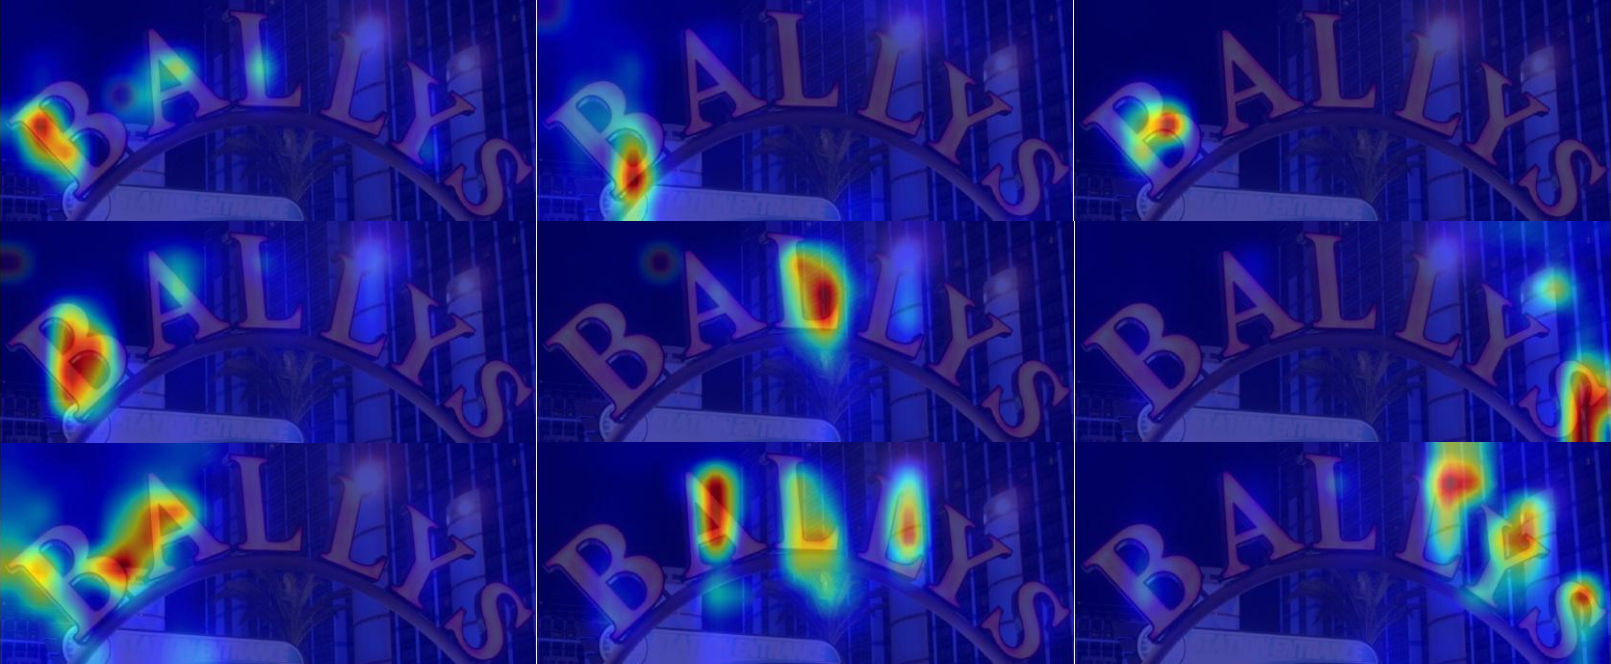
\includegraphics[width=\textwidth]{assets/visualization-of-svtr-attention-maps.png}
		\caption{Vizualizacija SVTR mapi pažnje}
		\label{fig:visualization-of-svtr-attention-maps}
	\end{figure}
	
	Svaka mapa se može objasniti kao da ima različitu ulogu u celokupnom prepoznavanju. Ilustracija devet primera mapa je prikazana na (Slici \ref{fig:visualization-of-svtr-attention-maps}). Prvi red prikazuje tri mape koje se fokusiraju na deo karaktera ``B'', sa naglaskom na njegovu levu stranu, donji deo i srednji deo, redom. Te tri mape ukazuju na to da različiti regioni karaktera doprinose njegovom prepoznavanju. Drugi red prikazuje tri mape koje se fokusiraju na različite karaktere, tj. ``B'', ``L'' i ``S''. SVTR takođe može da nauči karakteristike karaktera posmatrajući karakter kao celinu. Treći red prikazuje tri mape koje istovremeno aktiviraju više karaktera, što implicira da su zavisnosti među različitim karakterima uspešno uhvaćene. Ova tri reda zajedno otkrivaju da prepoznavač hvata tragove na nivou dela karaktera, celog karaktera i više karaktera, u skladu sa tvrdnjom da SVTR percipira višeslojne karakteristike komponenti karaktera, potvrđujući efikasnost SVTR-a.
	\newpage
	
	\section{Primene}
	Sistem za automatsko prepoznavanje teksta sa tablica vozila (ANPR) predstavlja inovativnu tehnologiju koja se sve više integriše u različite aspekte svakodnevnog života i upravljanja saobraćajem. Ova tehnologija omogućava brzo i precizno očitavanje registarskih oznaka vozila, što otvara brojne mogućnosti primene u različitim sektorima. Korišćenjem ANPR sistema, moguće je unaprediti efikasnost naplate putarina, automatski pratiti i locirati ukradena vozila, kao i optimizovati procese parkiranja i upravljanja kolinom vozila. 
	
	Pored toga, ANPR može igrati ključnu ulogu u poboljšanju bezbednosti saobraćaja, omogućavajući automatsku kontrolu saobraćajnih prekršaja i identifikaciju vozila koja su uključena u kriminalne aktivnosti. U kontekstu pametnih gradova, ova tehnologija može doprineti održivijem urbanom razvoju kroz efikasnije upravljanje saobraćajem i smanjenje zagađenja. S obzirom na sve ove prednosti, implementacija sistema za automatsko prepoznavanje registarskih tablica postaje ne samo korisna, već i neophodna za modernizaciju i unapređenje infrastrukture i usluga u urbanim sredinama. U ovom radu biće razmotrene različite primene ANPR sistema, kao i potencijalni izazovi i rešenja u njegovoj implementaciji.
	
	\subsection{Automatska naplata parkiranja}
	ANPR predstavlja značajan napredak u sistemima za naplatu parkiranja, omogućavajući bržu, efikasniju i korisniku prijatniju uslugu. Ova tehnologija omogućava automatsko očitavanje registarskih oznaka vozila prilikom ulaska i izlaska sa parking prostora, čime se eliminiše potreba za fizičkim karticama ili novčanim transakcijama na licu mesta. 
	
	Korišćenjem ANPR sistema, korisnici mogu jednostavno parkirati svoje vozilo bez dodatnog čekanja, dok se naplata vrši automatski putem unapred registrovanih podataka o vozilu. Ovo ne samo da smanjuje gužve na parking mestima, već i poboljšava korisničko iskustvo, čime se povećava zadovoljstvo vozača. Pored toga, ovakvi sistemi omogućavaju efikasnije upravljanje parking kapacitetima, jer pružaju ažurne informacije o zauzetosti parkinga, što može pomoći u optimizaciji korišćenja prostora. 
	
	Dodatno, ANPR tehnologija može doprineti smanjenju prevara i zloupotreba, jer se automatski evidentiraju svi ulazi i izlazi vozila, čime se povećava sigurnost i transparentnost u procesu naplate. Sve ove prednosti čine automatsko prepoznavanje registarskih tablica ključnim elementom modernih sistema za naplatu parkiranja, koji se sve više koriste u urbanim sredinama.
	
	\subsection{Automatska naplata putarine}
	ANPR može značajno unaprediti sistem automatske naplate putarina. ANPR sistem omogućava brzo i precizno očitavanje registarskih oznaka vozila prilikom prolaska kroz naplatne stanice, čime se eliminiše potreba za zaustavljanjem i fizičkim plaćanjem. Kao rezultat toga, vozači mogu nesmetano prolaziti kroz naplatne rampe, što smanjuje gužve i poboljšava protok saobraćaja na putevima.
	
	Korišćenjem ANPR tehnologije, naplata putarine postaje efikasnija i transparentnija, jer se automatski evidentiraju podaci o svakom vozilu, uključujući vreme prolaska i iznos naplate. Ovaj sistem takođe omogućava lakše praćenje i upravljanje naplatom, smanjujući mogućnost grešaka i prevara. Pored toga, ANPR može pomoći u identifikaciji vozila koja su prijavljena kao ukradena, čime se dodatno povećava bezbednost na putevima.
	
	\subsection{Automatsko praćenje i lociranje ukradenih vozila}
	ANPR omogućava efikasno praćenje i lociranje ukradenih vozila. Ovaj sistem omogućava brzu identifikaciju registarskih oznaka vozila u realnom vremenu, čime se nadležnim organima pruža mogućnost da odmah reaguju na prijave o ukradenim vozilima. Kada ANPR kamere prepoznaju registarsku tablicu koja se nalazi na listi ukradenih vozila, automatski se šalje obaveštenje nadležnim organima, čime se povećava šansa za brzo pronalaženje i vraćanje vozila vlasnicima. Osim što poboljšava efikasnost policijskih operacija, ANPR tehnologija takođe može pomoći u smanjenju stope kriminala, jer deluje kao odvraćajući faktor za potencijalne počinioce.
	
	\subsection{Automatska kontrola saobraćajnih prekršaja}
	ANPR olakšava precizno evidentiranje različitih prekršaja u realnom vremenu. Ova tehnologija omogućava automatizovano prepoznavanje registarske oznake vozila koja krše saobraćajne propise, kao što su prekoračenje brzine, prolazak kroz crveno svetlo ili nepropisno parkiranje. Kada se prekršaj zabeleži, sistem automatski generiše obaveštenje ili kaznu koja se šalje vlasniku vozila, čime se pojednostavljuje proces naplate kazni.
	
	Jedna od ključnih prednosti ANPR sistema je njegova sposobnost da smanji subjektivnost u procesu kontrole saobraćaja. Automatska identifikacija prekršaja omogućava doslednu primenu zakona, što može doprineti povećanju bezbednosti na putevima. Pored toga, ANPR može pomoći u prikupljanju podataka o saobraćajnim tokovima i obrascima ponašanja vozača, što omogućava vlastima da bolje planiraju saobraćajnu infrastrukturu i strategije prevencije.
	
	U javnom prevozu, ALPR može pomoći u praćenju i regulisanju vozila koja koriste specijalizovane trake, kao što su trake za autobuse ili taksi vozila, osiguravajući da ih koriste samo ovlašćena vozila. Ovo može doprineti efikasnijem funkcionisanju javnog prevoza i smanjenju zagušenja na putevima.
	
	Korišćenjem ANPR tehnologije, moguće je stvoriti efikasniji sistem kontrole saobraćaja koji smanjuje broj prekršaja i podstiče vozače da se pridržavaju saobraćajnih pravila. U svetlu ovih prednosti, jasno je da automatsko prepoznavanje registarskih tablica igra ključnu ulogu u unapređenju bezbednosti saobraćaja i smanjenju rizika od saobraćajnih nesreća.
	
	\subsection{Automatska kontrola pristupa}
	ANPR pruža efikasnu kontrolu i povećava bezbednost pristupa određenim zonama ili objektima. Ovakav sistem može biti od velike koristi u kontroli pristupa ekološkim zonama u gradovima, gde se ograničava pristup vozilima koja ne ispunjavaju ekološke standarde. Automatsko prepoznavanje registarskih tablica omogućava brzu identifikaciju takvih vozila i sprečavanje njihovog ulaska u zaštićene zone, čime se doprinosi smanjenju zagađenja i poboljšanju kvaliteta vazduha.
	
	Korišćenjem ANPR tehnologije, moguće je stvoriti fleksibilne i efikasne sisteme kontrole pristupa koji se mogu prilagoditi specifičnim potrebama svake zone ili objekta. Ova tehnologija predstavlja ključni element u unapređenju bezbednosti i upravljanju pristupom u savremenim urbanim sredinama.
	Može se koristiti za automatsko otvaranje kapija ili rampi u stambenim kompleksima ili poslovnim prostorima.
	
	Jedna od inovativnih primena ANPR tehnologije je u automatizovanim autoperionicama, gde se prepoznavanje registarskih tablica može koristiti za pružanje personalizovane usluge pranja vozila. Ovaj sistem može zapamtiti prethodne posete i preferencije klijenata, omogućavajući im da dobiju uslugu prilagođenu njihovim potrebama bez potrebe za dodatnim informacijama. Na taj način, klijenti mogu uživati u bržem i efikasnijem procesu pranja, dok autoperionice mogu optimizovati svoje operacije i poboljšati korisničko iskustvo.
	
	U stambenim ili garažnim zgradama koje imaju rezervisana parking ili garažna mesta, ANPR tehnologija eliminiše potrebu za više daljinskih upravljača za podizanje rampe i otvaranje garažnih vrata. Ovaj sistem omogućava automatsko otvaranje na osnovu prepoznate registarske tablice, čime se smanjuje upotreba plastike i doprinosi očuvanju životne sredine. Osim toga, korisnici više ne moraju da se obavezuju da nose više daljinskih upravljača, što dodatno olakšava svakodnevno korišćenje i povećava praktičnost.
	
	\subsection{Automatska kontrola saobraćaja}
	ALPR može imati ključnu ulogu u automatizovanoj kontroli saobraćaja, pružajući brojne prednosti za hitne službe i javni prevoz. Ova tehnologija može značajno poboljšati brzinu reakcije hitnih službi, kao što su ambulante, vatrogasci i policija, omogućavajući im brži dolazak na lice mesta. ALPR može prepoznati vozila hitnih službi i automatski otvoriti posebne saobraćajne trake ili raskrsnice, čime se smanjuje vreme potrebno za prolazak kroz gust saobraćaj. Ova funkcionalnost može biti od vitalnog značaja u situacijama kada je svaka sekunda važna, čime se potencijalno spašavaju životi.
	
	U kontekstu javnog prevoza, ALPR može pratiti i optimizovati rute autobusa i drugih prevoznih sredstava, čime se povećava tačnost i efikasnost servisa za obaveštavanje putnika o lokaciji i vremenu dolaska. Ova tehnologija omogućava prikupljanje podataka o saobraćajnim tokovima, što može pomoći u analizi i unapređenju rasporeda vožnje, čime se poboljšava iskustvo putnika.
	\newpage
	
	\section{Prikupljanje i rad sa podacima}
	U ovom poglavlju biće objašnjene metode prikupljanja podataka, izazovi sa kojima se istraživači susreću tokom ovog procesa, kao i značaj obrade i pripreme podataka za dalji rad na razvoju sistema za prepoznavanje teksta sa registarskih tablica.
	
	\subsection{Uvod u prikupljanje podataka}
	Osnovu za razvoj sistema za automatsko prepoznavanje teksta sa tablica čini kvalitetan i obiman skup podataka. Prikupljanje ovih podataka predstavlja jedan od ključnih koraka u procesu razvoja takvog sistema, jer direktno utiče na uspešnost i preciznost modela za prepoznavanje. Zbog toga je neophodno posvetiti posebnu pažnju metodama i tehnikama koje se koriste za prikupljanje podataka, kao i izazovima koji mogu nastati u ovom procesu.
	
	Prikupljanje podataka podrazumeva sakupljanje slika registarskih tablica iz različitih izvora, koje će se koristiti za treniranje, validaciju i testiranje modela. Kvalitet prikupljenih podataka, njihova reprezentativnost i raznovrsnost igraju ključnu ulogu u postizanju visokih performansi sistema za prepoznavanje teksta. Osim toga, treba uzeti u obzir i pravne aspekte i zaštitu privatnosti, jer rad sa podacima koji sadrže informacije o vozilima može biti podložan strogoj regulativi.
	
	\subsection{Specifičnosti prikupljanja podataka u kontekstu prepoznavanja teksta sa registarskih tablica}
	\begin{figure}[H]
		\centering
		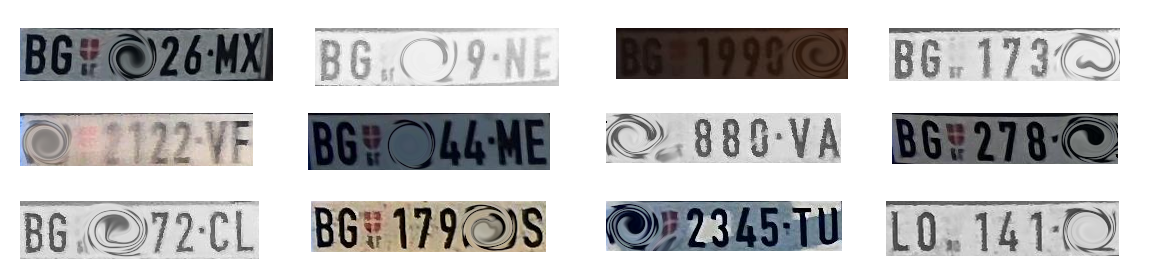
\includegraphics[width=\textwidth]{assets/license-plate-samples.png}
		\caption{Primeri tablica iz skupa realnih podataka. Svi priloženi primeri tablica su svesno oštećeni kako bi se sačuvala anonimnost i privatnost osoba čije tablice su prikazane.}
		\label{fig:license-plate-samples}
	\end{figure}
	
	\subsubsection{Varijabilnost registarskih tablica}
	\paragraph{Raznolikost dizajna}
	Registarske tablice variraju od zemlje do zemlje, pa čak i unutar iste države, u pogledu boje, fonta, veličine slova, rasporeda karaktera i prisustva simbola ili grbova. Ova raznolikost zahteva prikupljanje podataka koji obuhvataju širok spektar različitih tablica kako bi model bio sposoban da prepozna sve varijante.
	
	\paragraph{Fizičko stanje tablica}
	Tokom vremena, registarske tablice mogu postati oštećene, izbledele ili prljave, što može otežati prepoznavanje teksta. Prikupljanje slika sa različitim stepenima oštećenja tablica je ključno za treniranje modela koji može da se nosi sa takvim izazovima.
	
	\subsubsection{Promenljivi uslovi snimanja}
	\paragraph{Različiti uslovi osvetljenja}
	Snimanje registarskih tablica može se odvijati u različitim vremenskim uslovima i periodima dana, što rezultira varijacijama u osvetljenju. Sakupljanje podataka u različitim svetlosnim uslovima (npr. jaka sunčeva svetlost, senke, noćno snimanje) omogućava modelu da se prilagodi tim promenama (Slika \ref{fig:license-plate-samples}).
	
	Snimanje noću predstavlja poseban izazov zbog nedostatka prirodnog svetla. Kamere koje nemaju odgovarajuće noćne režime snimanja ili infracrveno osvetljenje mogu proizvesti slike lošeg kvaliteta sa dosta šuma. Dodatno, farovi vozila mogu uzrokovati probleme sa kontrastom i zaslepljivanjem, što dodatno otežava prepoznavanje tablica.
	
	\paragraph{Različiti uglovi snimanja}
	U zavisnosti od položaja kamere, registarske tablice mogu biti snimljene pod različitim uglovima, što može izazvati probleme sa perspektivnim izobličenjem. Kada kamera nije postavljena direktno ispred tablice, već pod određenim uglom, karakteri na tablici mogu izgledati iskrivljeno ili izduženo. Ovo posebno dolazi do izražaja u slučajevima kada kamere moraju biti montirane na nepristupačnim mestima, poput visokih stubova ili nadstrešnica, gde se tablice snimaju pod oštrim uglovima u odnosu na horizontalnu osu vozila.
	
	\paragraph{Kretanje vozila}
	Snimanje registarskih tablica vozila koja se kreću predstavlja izazov zbog potencijalnog zamagljenja slika. Kada se vozilo kreće, kamera mora da zabeleži sliku u vrlo kratkom vremenskom intervalu kako bi se izbeglo zamagljenje. koje može otežati prepoznavanje karaktera na tablici.
	
	\subsection{Upoznavanje sa podacima}
	Za razvoj sistema za automatsko prepoznavanje teksta sa registarskih tablica, postoji nekoliko javno dostupnih baza podataka koje sadrže slike tablica iz različitih zemalja. Ove baze podataka pružaju širok spektar slika sa različitim tipovima registarskih tablica, različitih kvaliteta i uslova snimanja, što ih čini korisnim za treniranje i evaluaciju modela za prepoznavanje teksta. Neki od najpoznatijih javno dostupnih skupova podataka uključuju:
		
	\paragraph{\href{https://github.com/raysonlaroca/ufpr-alpr-dataset}{UFPR-ALPR}}
	Baza podataka koja sadrži 4.500 slika registarskih tablica iz različitih zemalja. Ovaj skup podataka obuhvata tablice sa različitim fontovima, bojama i rasporedima karaktera.
	
	\paragraph{\href{https://github.com/detectRecog/CCPD}{CCPD (Chinese City Parking Dataset)}}
	Skup podataka koji se fokusira na kineske registarske tablice, ali može biti koristan kao referenca za treniranje modela sa slikama koje obuhvataju različite uslove osvetljenja i uglove snimanja.
	
	\paragraph{\href{https://datasetninja.com/car-license-plate}{Car License Plate Dataset}}
	Baza podataka sa oko 400 slika vozila i registarskih tablica, koja pokriva različite scenarije, uključujući vozila u pokretu, snimke iz različitih perspektiva, i različite vremenske uslove. \newline
	
	Međutim, iako ovi skupovi podataka mogu biti korisni za razvoj generalnih sistema za prepoznavanje teksta sa registarskih tablica, oni su ograničeni u pogledu specifičnosti dizajna i karakteristika registarskih tablica koje se koriste u Srbiji.
	
	S obzirom na to da sam se fokusirao na razvoj rešenja za prepoznavanje teksta sa srpskih registarskih tablica, kao i da imam pristup skupu od oko 17000 slika uglavnom Srpskih tablica sa ulaza ispred rampi, odlučio sam da se oslonim prvenstveno na ove specifične podatke. Ovaj pristup omogućava treniranje modela koji je prilagođen karakteristikama srpskih tablica, kao što su specifičan font, raspored karaktera i prisustvo nacionalnih simbola. Dodatno, slike snimljene na ulazima ispred rampi pružaju realne scenarije sa kojima će se model susretati u stvarnim aplikacijama, što dodatno povećava relevantnost i pouzdanost razvijenog rešenja.
	
	\subsection{Razvrstavanje i čišćenje podataka}
	Nakon prikupljanja, sledi faza čišćenja podataka, koja podrazumeva identifikaciju i uklanjanje nekvalitetnih ili irelevantnih slika. Na primer, slike koje su previše zamagljene, oštećene, ili ne sadrže jasno vidljive registarske tablice, moraju biti uklonjenje iz skupa podataka. Ova faza obezbeđuje da model bude treniran na kvalitetnim i relevantnim podacima, što utiče na njegovu tačnost i robusnost.
	
	Na kraju, pripremljeni podaci se dele u grupe za treniranje, validaciju i test. Grupa podataka za treniranje se koristi za obučavanje modela, grupa podataka za validaciju korisna je za podešavanje hiperparametara i evaluaciju performansi tokom treniranja, dok se test grupa podataka koristi za konačnu procenu modela nakon treniranja. Pravilna podela podataka je ključna za izbegavanje prekomerne prilagođenosti i osiguranje da model može dobro da generalizuje na novim, neviđenim podacima.
	
	\subsection{Anotacija podataka}
	Anotacija predstavlja označavanje delova slike koji sadrže ključne regije, u ovom slučaju registarske tablice i tekst koji je ispisan na tablicama. Anotacija podataka je proces u kojem se ručno ili poluautomatski označavaju tačne lokacije i sadržaj registarskih tablica na svakoj slici. U ovoj fazi se koristi softver za anotaciju, koji omogućava obeležavanje granica tablica i unos odgovarajućeg teksta. Kvalitetna anotacija je veoma bitna jer direktno utiče na uspešnost treniranja modela. Greške u anotaciji, poput netačnih ili nepotpunih oznaka, mogu dovesti do smanjenja tačnosti modela i takav tip greške se kasnije vrlo teško pronalazi.
	
	\subsection{Kreiranje sintetičkog skupa podataka}
	Kreiranje sintetičkog skupa podataka pomaže uvećanju inicijalnog skupa i posebno je od značaja kada je dostupnost realnih podataka ograničena.
	
	\subsubsection{Prednosti sintetičkih podataka}
	Sintetički skup podataka omogućavaju stvaranje velike količine podataka bez potrebe za obimnim prikupljanjem i anotacijom realnih slika, što može biti vremenski i finansijski zahtevno. Sintetički podaci omogućavaju preciznu kontrolu nad svim aspektima slike, uključujući osvetljenje, ugao snimanja, pozadinu, i stil registarskih tablica(izbor fonta, veličine, boje i pozicije teksta, i slično). Ovo omogućava modelu da se obučava na širokom spektru varijacija, čime se povećava njegova robusnost i otpornost na različite uslove snimanja.
	
	Sintetički skupovi podataka takođe omogućavaju simulaciju retkih ili ekstremnih slučajeva, kao što su tablice sa specifičnim oštećenjima, delimično zaklonjene tablice, ili tablice snimljene u nepovoljnim vremenskim uslovima. Kreiranjem ovakvih slika, model može biti pripremljen za situacije koje se možda neće često pojavljivati u realnim podacima, ali su ipak važne za sveobuhvatnu tačnost sistema.
	
	\subsubsection{Generisanje pozadina tablica}
	\begin{figure}[H]
		\centering
		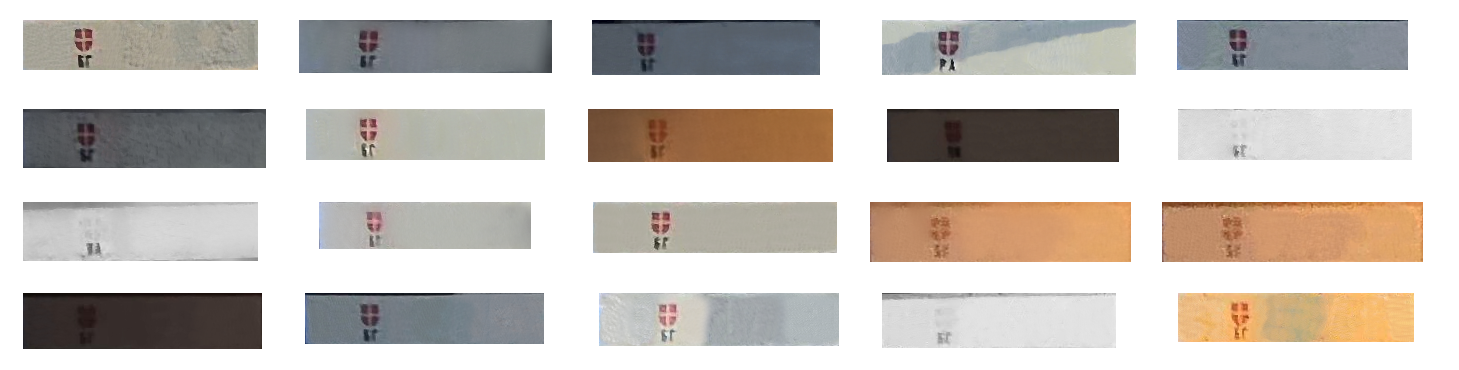
\includegraphics[width=\textwidth]{assets/license-plate-backgrounds.png}
		\caption{Primeri generisanih pozadina tablica}
		\label{fig:license-plate-backgrounds}
	\end{figure}
	
	Za generisanje pozadina tablica, odlučio sam da koristim slike stvarnih registarskih tablica kako bih postigao visok nivo autentičnosti. Prvo sam odabrao nekoliko slika pravih tablica, snimljenih u različitim uslovima, kako bih obezbedio raznovrsnost u teksturi, boji i detaljima. Zatim sam, koristeći GIMP, obrisao sve karaktere sa tih slika, zadržavajući osnovnu strukturu i karakteristike tablice netaknute. Na ovaj način imao sam čiste pozadine koje izgledaju prirodno i verodostojno (Slika \ref{fig:license-plate-backgrounds}).
	
	\subsubsection{Generisanje teskta na tablicama}
	\begin{figure}[H]
		\centering
		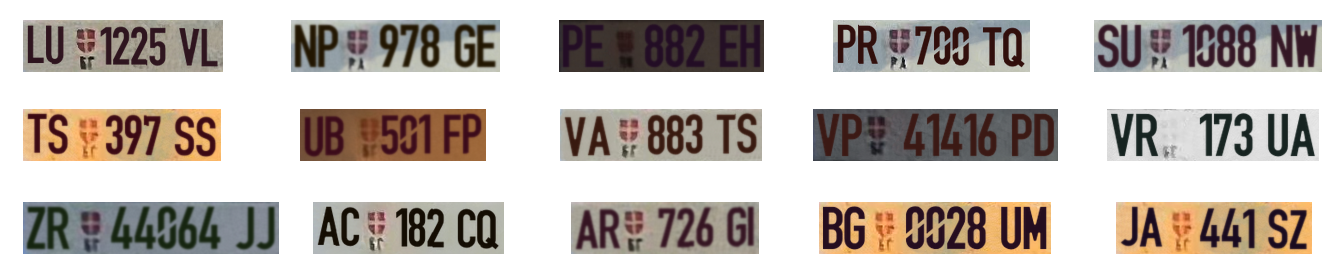
\includegraphics[width=\textwidth]{assets/synthetic-license-plates.png}
		\caption{Primeri sintetičkog skupa podataka}
		\label{fig:synthetic-license-plates}
	\end{figure}
	
	Nakon generisanja pozadina tablica, koristio sam repozitorijum \href{https://github.com/Belval/TextRecognitionDataGenerator}{TextRecognitionDataGenerator}, koji sam modifikovao kako bih mogao da na tačno određenim mestima i pod odgovarajućim uglovima dodajem tekst na generisane pozadine tablica. Prethodno sam generisao tekst u skladu sa pravilima za izradu registarskih tablica u Republici Srbiji, vodeći računa da kontekst bude validan. Ovako prilagođena verzija alata uz korišćenje specijalno izrađenog fonta omogućila mi je da kreiram sintetički skup tablica koje podsećaju na stvarne srpske tablice (Slika \ref{fig:synthetic-license-plates}).
	
	\subsubsection{Integracija sintetičkih podataka sa realnim podacima}
	Kada se kreira sintetički skup podataka, bitno je integrisati ga sa realnim podacima tako da bude postignut optimalan balans između realističnosti i varijabilnosti. Sintetički podaci mogu se koristiti kao dodatak realnim podacima, čime se povećava veličina i raznovrsnost skupa podataka za treniranje. Kombinovanjem sintetičkih i realnih podataka, model može naučiti kako da prepoznaje tekst sa registarskih tablica u različitim scenarijima, dok istovremeno ostaje veran stvarnim uslovima koje će susretati u praksi.
	
	\subsection{Augmentacija podataka}
	Kako bi se povećala raznovrsnost skupa podataka i model bolje prilagodio različitim uslovima snimanja, često se primenjuje tehnika augmentacije podataka. Augmentacija podrazumeva generisanje novih slika iz postojećih putem različitih transformacija, kao što su rotacija, promena osvetljenja, skaliranje, i dodavanje šuma. Ove transformacije omogućavaju simulaciju različitih realnih uslova, poput snimanja pod različitim uglovima, promena u osvetljenju, ili prisustva šuma na slici. Na ovaj način se model obučava na većem broju različitih scenarija, što doprinosi njegovoj otpornosti na varijacije u podacima.
	
	\subsection{Podela podataka}
	Prilikom treniranja modela dostupni skup podataka je potrebno podeliti u tri distinktivna podskupa: trening skup, validacioni skup i test skup. Ovakva podala podataka, gde se jedan podatak, u ovom slučaju slika, nalazi isključivo samo u jednom od tri skupa je fundamentala za razvoj, evaluaciju i verifikaciju modela.
	
	Trening skup čini najveći deo inicijalnog skupa podataka(obično od 60-80\%), koristi se za obučavanje modela. Koristeći podatke iz trening skupa model uči obrasce, relacije i karakteristike koje su svojstvene problemu koji se rešava.
	
	Validacioni skup je manji i obično oko 10-20\% inicijalnog skupa podataka. Služi za finu kalibraciju modela i sprečavanje prekomerne prilagođenosti modela trening skupu tokom treninga. Koristi se i za procenu performanci modela tokom faze obuke i za podešavanje hiperparametara.
	
	Test skup je finalni podskup koji čini oko 10-20\% inicijalnih podataka i koristi se za nezavisnu evaluaciju konačnog modela. Ovaj skup ostaje nekorišćen do završetka treninga i kalibracije, čime se obezbeđuje objektivna procena generalizacijske sposobnosti modela na novim, prethodno neviđenim podacima.
	
	Ovakva metodologija podele podataka omogućava razvoj robusnih modela koji imaju veću pouzdanost i praktičnu primenljivost u realnim scenarijima.
	
	\subsection{Opis korišćenog skupa podataka}
	Skup realnih podataka koje sam koristio za proces treniranja modela sadržao je 5.838 slika pravih srpskih tablica, uglavnom registrovanih u Beogradu. Sve slike su pažljivo označene i višestruko proverene kako bi se izbeglo propuštanje nepravilno označenih podataka, što bi dovelo do loših rezultata prilikom treninga modela. Uzevši u obzir mali broj dostupnih slika za trening, augmentacijom i pravljenjem sintetičkih podataka povećao sam skup podataka sa 5.838 na 124.838 slika. Prilikom augmentacije i pravljenja sintetičkih podataka inicijalni skup sam obogatio sa slikama različitih scenarija vremenskih i dnevnih uslova, kao i različitim uglovima slikanja kamere. Pored toga što doprinosi varijabilnosti uslova osvetljenja i kvantitetu podataka, dodavanje sintetičkog skupa unosi i novi kontekst teksta na tablicama, gde sam u sintetičkom skupu napravio primere tablica koje su mogle biti registrovane u \href{https://www.super-registracija-vozila.rs/registarske-oznake-u-srbiji}{ostalim dozvoljenim gradovima} u Srbiji pored Beograda. Dobra strana rada sa sintetičkim podacima jeste i to što nisam imao ručnu fazu označavanja podataka.
	\newpage
	
	\section{Implementacija}	
	Kako bih sa veoma velikom sigurnošću mogao da radim prepoznavanje teksta sa tablica automobila, napravio sam servis za automatizovano prepoznavanje teksta sa tablica ulaznih slika koristeći modele za detekciju tablica i teksta sa scene. Ovaj pristup omogućava preciznije i pouzdanije rezultate, jer se oslanja na kombinaciju različitih modela koji su specijalizovani za različite aspekte prepoznavanja regija od važnosti.
	
	\subsection{Dodatne komponente sistema}
	Ono što se pokazalo kao zanimljiv izazov u ovom procesu je to što nije bilo dovoljno koristiti samo model za detekciju tablica. Mnoge registarske tablice imaju dodatne elemente, poput reklama ili natpisa na okvirima, koji mogu ometati proces prepoznavanja teksta. Da bi se postigla visoka tačnost u prepoznavanju teksta sa registarskih oznaka, bilo je neophodno razviti metodologiju koja će eliminisati takve neželjene informacije pre nego što se pređe na prepoznavanje teksta sa registarskih oznaka.
	
	S druge strane, korišćenje modela isključivo za detekciju teksta nije prihvatljivo kao robusno rešenje. Na slikama na kojima se nalaze registarske tablice često se može naći i drugi tekst koji ne predstavlja tablicu, kao što su natpisi, reklame, ime brenda automobila ili drugi elementi iz okruženja. Ako bi se oslonio isključivo na model za detekciju teksta, postojala bi dosta velika verovatnoća da će model pogrešno identifikovati ili obraditi neželjene informacije, što bi moglo dovesti do netačnih rezultata.
	
	Zbog toga je servis dizajniran tako da prvo detektuje tablice na ulaznim slikama, a zatim koristi model za prepoznavanje teksta isključivo unutar detektovanih oblasti tablica. Na ovaj način mogu efektivno da izbacim tekst koji je ispisan po okvirima ili značajno fontom u odnosu na glavni tekst koji se nalazi duž tablice.
	
	\subsubsection{Detektor tablica}
	Model koji sam koristio za detekciju tablica je \href{https://huggingface.co/nickmuchi/yolos-small-finetuned-license-plate-detection}{YOLOS vizuelni transformer} \cite{fang2021looksequencerethinkingtransformer} inicijalno treniran na ImageNet skupu podataka i fino podešen kroz 200 epoha na skupu od \href{https://universe.roboflow.com/objectdetection-jhgr1/license-plates-recognition/dataset/2}{5200 slika tablica}.
	
	Ovaj model je razvijen kako bi poboljšao efikasnost i preciznost detekcije objekata koristeći transformere umesto tradicionalnih konvolucionih mreža.
	
	YOLOS se oslanja na arhitekturu vizuelnog transformera koja omogućava modelu da obrađuje slike kao nizove vizuelnih tokova. Sa tim pristupom model može da uoči dugoročne zavisnosti i kompleksne obrasce u slikama, što poboljšava tačnost detekcije objekata.
	
	Ono što izdvaja YOLOS je jednostavnost dizajna modela, koja omogućava postizanje visokih performansi u detekciji objekata uz relativno manji broj slojeva i parametara u poređenju sa drugim transformator modelima.
	
	\subsubsection{Detektor teksta}
	Za detekciju teksta na sceni sam koristio \href{https://github.com/clovaai/CRAFT-pytorch?tab=readme-ov-file}{CRAFT} model koji je osmišljen da poboljša prepoznavanje i lokalizaciju teksta u složenim slikama koristeći dve glavne komponente: Svest o oblasti i klasifikaciju karaktera.
	
	Deo modela zadužen za svest o oblasti se fokusira na identifikaciju i precizno lokalizovanje područja na slici gde se mogu nalaziti karakteri, omogućavajući modelu da prepozna različite oblike i orijentacije teksta. Dok deo vezan za klasifikaciju karaktera koristi karakteristične informacije za klasifikaciju prepoznatih regija i precizno identifikuje pojedinačne karaktere \cite{baek2019characterregionawarenesstext}.
	
	\subsection{Metodologije i tehonologije korišćene u razvoju servisa}
	\subsubsection{PaddlePaddle}
	\href{https://github.com/PaddlePaddle}{PaddlePaddle} je open-source framework za duboko učenje koji je razvijen od strane Baidu-a. Jedan je od najpopularnijih projekata na GitHub-u koji se bave mašinskim učenjem, a PaddlePaddleOCR deo je trenutno i najpopularniji repozitorijum na temu optičkog prepoznavanja karaktera.
	
	PaddlePaddleOCR projekat pruža veliki broj implementiranih modela iz aktuelnih radova koji se bave prepoznavanjem teksta sa slika. Ovi modeli pokrivaju širok spektar OCR zadataka, uključujući prepoznavanje teksta na različitim jezicima, analizu strukture dokumenata, prepoznavanje formula i tabela, kao i druge specijalizovane primene.
	
	Pored implementacije najnaprednijih OCR modela, Paddle pruža i alate za anotaciju podataka, generisanje sintetičkih slika za trening, kao i optimizaciju i ubrzanje modela za efikasnu primenu na različitim platformama - od servera do mobilnih uređaja i ugrađenih sistema.
	
	Kao početnu tačku za implementaciju prepoznavanja teksta sa tablica automobila sam koristio njihovu impelemtaciju SVTR modela.
	
	\subsubsection{Upravljanje pristupom servisu}
	Kako bi prepoznavanje tablica moglo da se koristi kao servisna aplikacija, koristio sam \href{https://www.uvicorn.org/}{Uvicorn} i \href{https://fastapi.tiangolo.com/}{FastAPI} za izradu web servisa i otvorio rutu za pristup servisu. FastAPI je moderan i brz web framework za pravljenje API-ja u Python programskom jeziku i omogućava lako definisanje ruta i automatsku validaciju podataka. Njegova sposobnost da generiše interaktivnu dokumentaciju putem Swagger-a čini ga izuzetno korisnim za razvoj i testiranje API-ja.
	
	Uvicorn je performantni ASGI server koji podržava asinhrono rukovanje zahtevima. Njegova integracija sa FastAPI-jem omogućava efikasno upravljanje višestrukim pozivima i događajima, što je ključno za aplikacije koje zahtevaju brze i responzivne interakcije sa korisnicima. 
	
	Za pristup servisu za prepoznavanje teksta sa tablica sam otvorio rutu pod nazivom \enquote{/do\_lpr}, koja prihvata sliku kao ulaz. Izlaz iz ove rute su isečena slika tablice sa inicijalne slike i pročitani tekst sa tablice. Na ovaj način korisnici treba samo da pošalju sliku na kojoj se nalazi registarka tablica i za tu sliku će dobiti relevantne informacije.
	
	Korišćenje FastAPI-ja i Uvicorn-a mi je olakšalo i pravljenje dokumentacije, jer pruža automatski generisanu Swagger dokumentaciju na osnonvu ispisanog koda.
	
	\subsubsection{Distribuiranje i skaliranje}
	Servis koji sam napravvio sam odlučio da upakujem i distribuiram pomoću Docker-a. \href{https://www.docker.com/}{Docker} je platforma za kontejnerizaciju aplikacija koja omogućava lako kreiranje, distribuiranje i pokretanje aplikacija u izolovanom okruženju, poznatom kao kontejner.
	
	Jedan od glavnih razloga za korišćenje Docker-a je obezbeđivanje konzistentnog okruženja za rad aplikacije. Docker kontejneri garantuju da će aplikacija raditi isto na različitim mašinama, čime se eliminišu problemi sa zavisnostima i razlikama u okruženju. Zahvaljujući Docker-u, mogu biti siguran prilikom razvoja da će aplikacija funkcionisati bez obzira na to gde se pokreće, što značajno olakšava proces implementacije.
	
	Osim toga, Docker omogućava lako skaliranje i prenosivost aplikacija. Kontejneri su jednostavni za prenos između različitih platformi, što olakšava distribuciju i implementaciju servisa. Takođe, Docker pruža alate za efikasno upravljanje životnim ciklusom aplikacije, uključujući kreiranje, pokretanje, zaustavljanje i brisanje kontejnera.
	
	Docker, kao rešenje, omogućava isporuku robusnog, skalabilnog i lako upotrebljivog rešenja.
	\newpage
	
	\section{Rezultati}
	
	\subsection{Treniranje modela prepoznavanja teksta}
	Uzevši u obzir da sam imao pristup malom broju podataka čak i nakon odrađene augmentacije i dodavanja sintetičkog skupa, tokom treniranja neke od parametara sam ekperimentalnim pristupom podesio na sledeće vrednosti:
	\begin{itemize}
		\item Broj epoha: 50; Iako je broj epoha postavljen na 50, zbog malog broja dostupnih podataka model bi najčešće konvergirao u trenutku od druge do pete epohe.
		\item Korak za testiranje nad validacionim skupom: 200; Na svakih 200 završenih grupa podataka prilikom treninga pokreće se evaluacija nad validacionim skupom podataka.
		\item Stopa učenja: Koristio sam kosinusnu stopu učenja sa početnom vrednošću postavljenom na 0.0005.
		\item Veličina ulazne slike: širina 320px, visina 48px i 3 kanala boja(RGB).
	\end{itemize}
	
	Model za prepoznavanje teksta sam trenirao na KDE Neon Linux mašini sa sledećim specifikacijama:
	\begin{itemize}
		\item GPU: NVIDIA GeForce RTX 4080, 16GB VRAM
		\item CPU: 12th Gen Intel i7-12700KF
		\item RAM: 32GB
	\end{itemize}

	Za evaluaciju i praćenje treniranja modela koristio sam CTC(Connectionist Temporal Classification), NRTR(Non-Recurrent Text Recognition) i sumarni gubitak te dve funkcije. \href{https://paperswithcode.com/method/ctc-loss}{CTC gubitak} se koristi u primerima gde je usklađenost između ulaznih i izlaznih sekvenci nepoznata. Ulazne sekvence u ovom slučaju predstavljaju slike koje sadrže tekst, a izlazne sekvence predstavljaju niz karaktera koji je zapisan na slici. CTC omogućava modelu da generiše sekvencu verovatnoća za svaki karakter i predstavlja dobar pristup za različite dužine ulaznih i izlaznih sekvenci. Funkcija gubitka izračunava verovatnoću ispravne sekvence sabiranjem svih mogućih usklađenja, što omogućava modelu da uči iz neusklađenih podataka \cite{inproceedings}. NRTR gubitak je dizajniran za nerekurentne modele, posebno za modele bazirane na transformer arhitekturi. Efikasan je za duge sekvence, jer ima sposobnost paralelnog procesiranja \cite{hu2020gtcguidedtrainingctc}.
	
	\subsubsection{Treniranje koristeći samo realne podatke}
	\begin{figure}[H]
		\centering
		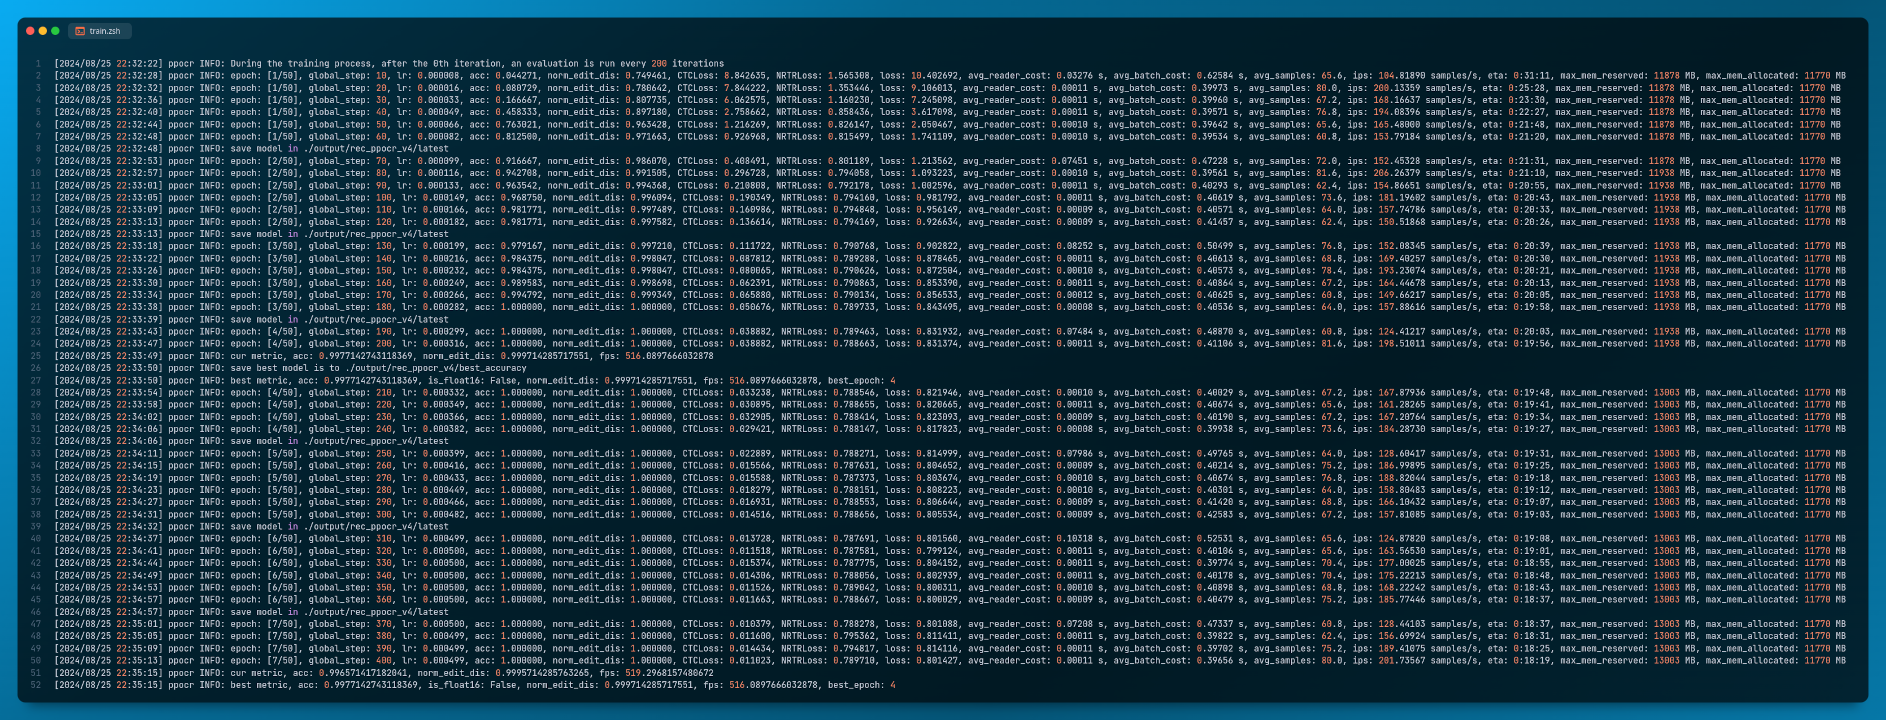
\includegraphics[width=\textwidth]{assets/train-code-real-data.png}
		\caption{Proces treniranja modela za detekciju teksta na realnim podacima}
		\label{fig:train-code-real-data}
	\end{figure}

	\begin{figure}[H]
		\centering
		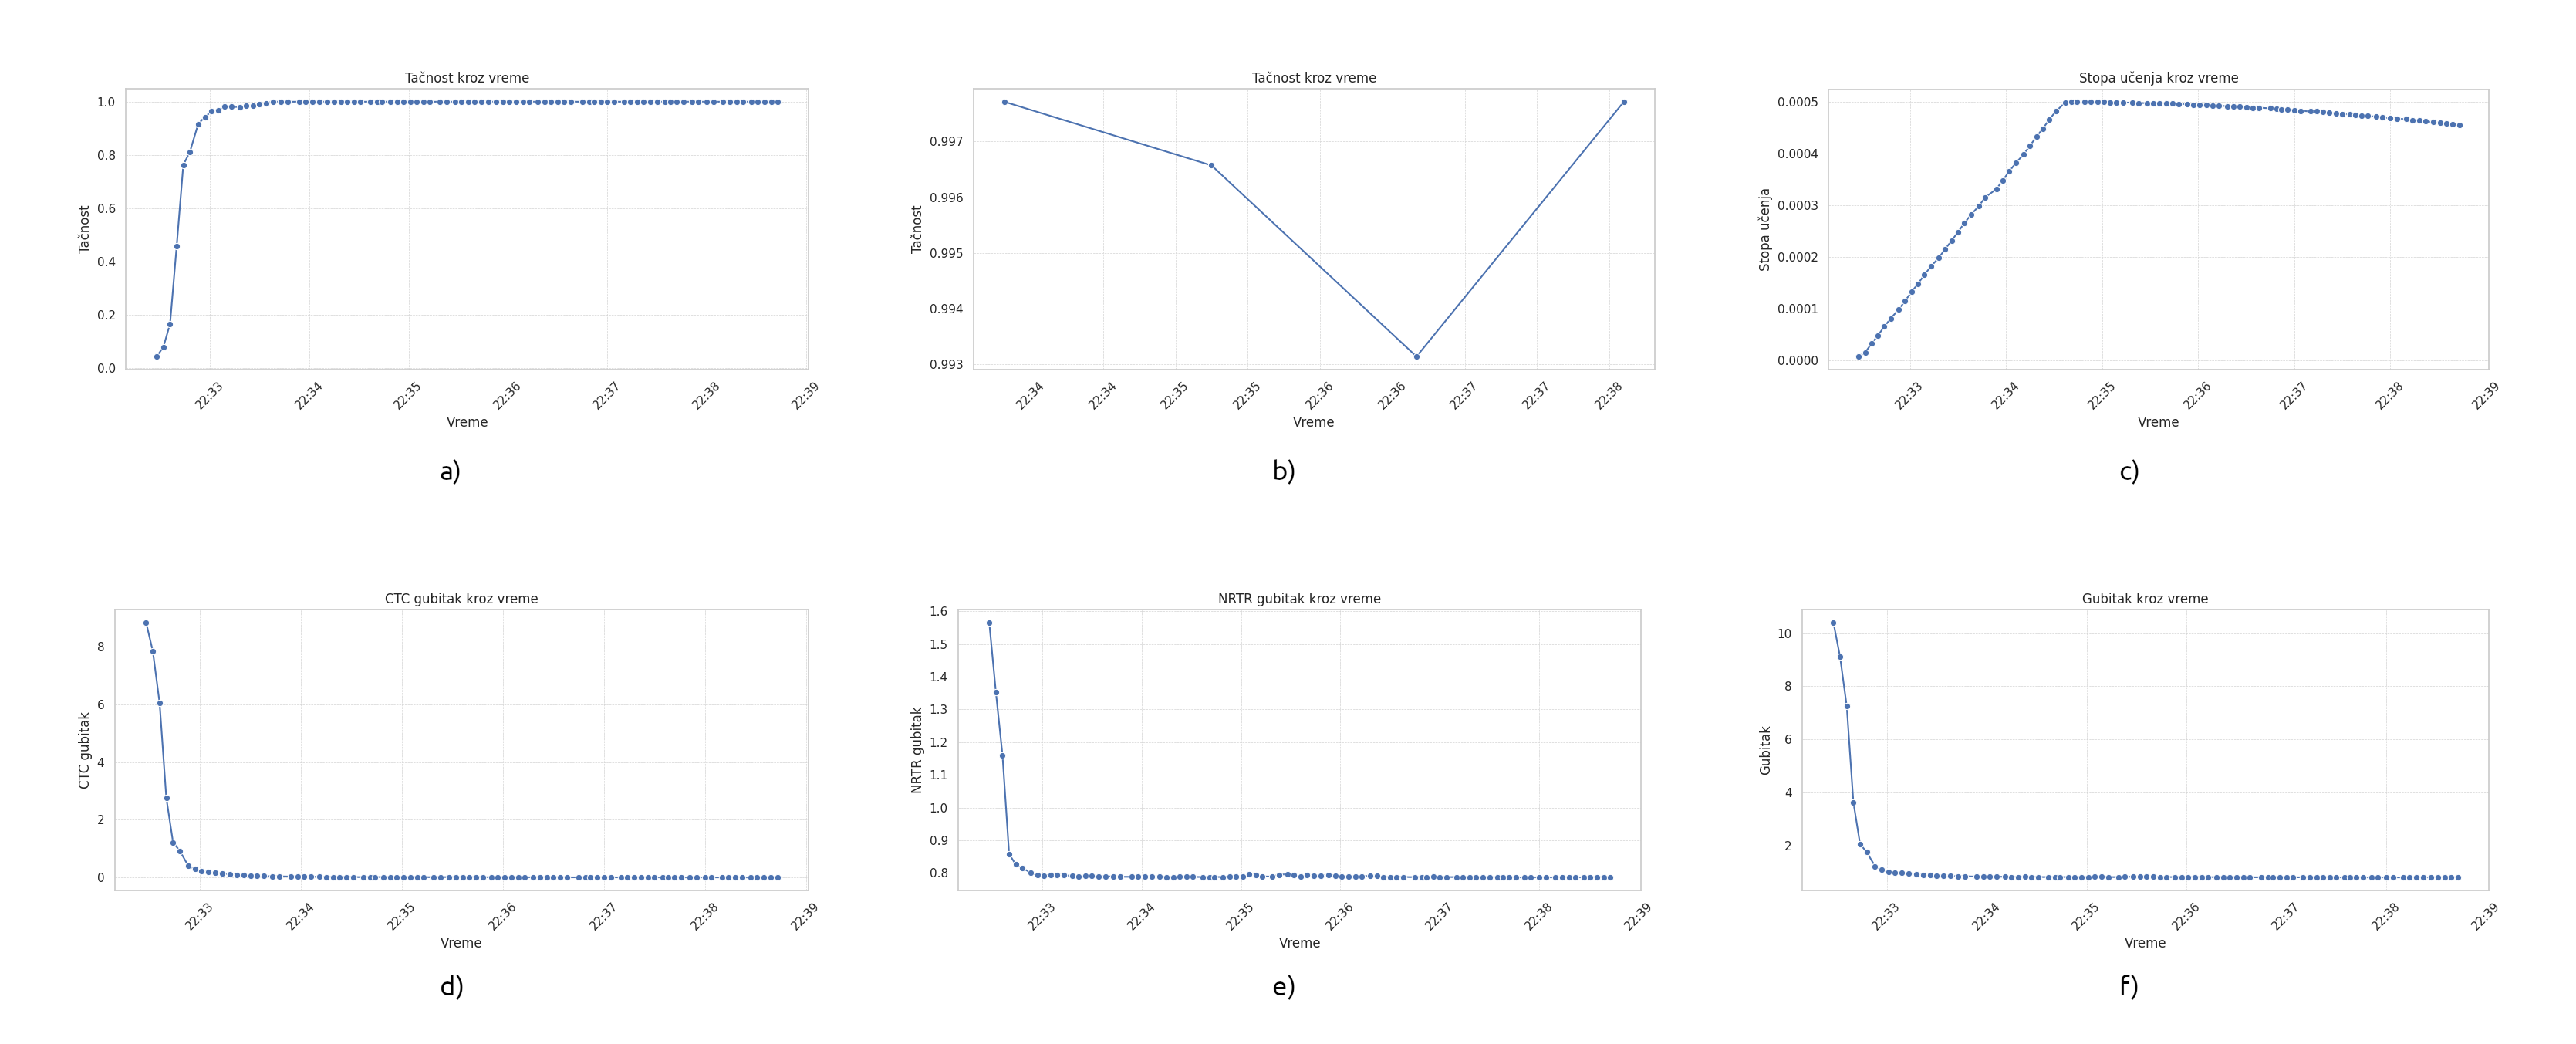
\includegraphics[width=\textwidth]{assets/real-data-metrics.png}
		\caption{Metrike u toku treniranja modela sa realnim podacima. a) Tačnost modela na trening podacima u toku obučavanja modela. b) Tačnost modela na validacionim podacima u toku obučavanja modela. c) Promena vrednosti stope učenja u toku obučavanja modela. d) CTC gubitak u toku obučavanja modela. e) NRTR gubitak u toku obučavanja modela f) Gubitak u toku obučavanja modela.}
		\label{fig:real-data-metrics}
	\end{figure}
	
	Imajući u vidu da sam za treniranje modela imao samo 5.838 realnih slika tablica automobila registrovanih uglavnom u Beogradu i koje su bile označene i proverene, trening je trajao samo par minuta. Model je konvergirao za nekoliko minuta i dostigao tačnost od 100\% (Slika \ref{fig:real-data-metrics}(a)) na trening skupu i 99.77\% (Slika \ref{fig:real-data-metrics}(b)) na validacionom skupu, koji je pomogao u usmeravanju treninga (Slika \ref{fig:train-code-real-data}).\newline
	
	Dostupni skup realnih podataka sam podelio u sledeće podskupove:
	\begin{itemize}
		\item Trening skup je činilo 70\% podataka, što je 4.086 slika
		\item Validacioni skup je činilo 15\% podataka, što je 875 slika
		\item Test skup je činilo 15\% podataka, što je 875 slika
	\end{itemize}
	
	Uzevši u obzir veoma visoku tačnost na trening i validacioinm podacima, najbitnija provera koja validira da li je model dobro istreniran ili je došlo do prekomerne prilagođenosti, jeste provera nad test skupom podataka. Uspešnost na nezavisnom testu nad skupom testnih podataka koje model nije mogao da vidi ni u jednom trenutku prilikom treniranja iznosi 100\%, što ukazuje na to da model nije imao problem sa prekomernom prilagođenosti podataka prilikom treniranja.
	
	Pored visoke tračnosti, model takođe ima i visok stepen sigurnosti prilikom predikcije, sa prosečnom sigurnošću od 99,91\% za svaku predikciju koju je izvršio na testnom skupu podataka.
	
	Međutim, obzirom na to da skup realnih podataka nije bio ni kontekstualno dovoljno raznovrstan, niti kvantitativno dovoljno veliki, treniranje nastavljam sa sintetičkim podacima.
	
	\subsubsection{Treniranje koristeći samo sintetičke podatke}
	Pre nego što odradim treniranje na spojenim skupovima realnih i sintetičkih podataka, želeo sam da proverim tačnost modela u scenariju u kojem nisam imao pristup realnim podacima tokom treninga, već sam morao da koristim isključivo sintetičke podatke.
	
	\begin{figure}[H]
		\centering
		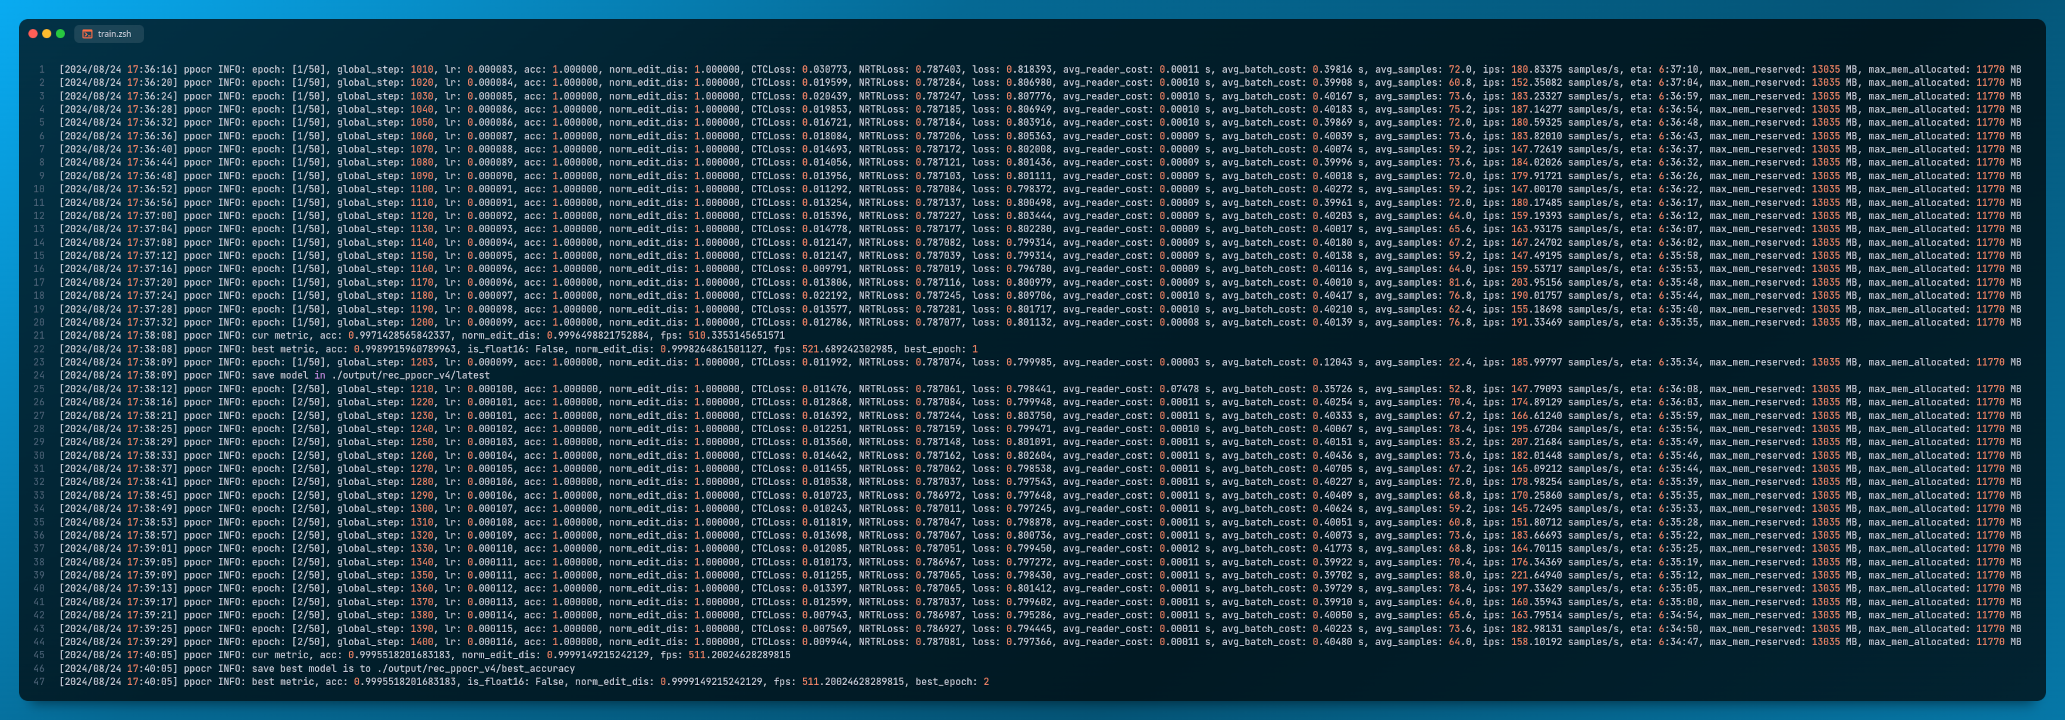
\includegraphics[width=\textwidth]{assets/train-code-synthetic-data.png}
		\caption{Krajnja faza procesa treniranja modela za detekciju teksta na sintetičkim podacima}
		\label{fig:train-code-synthetic-data}
	\end{figure}

	\begin{figure}[H]
		\centering
		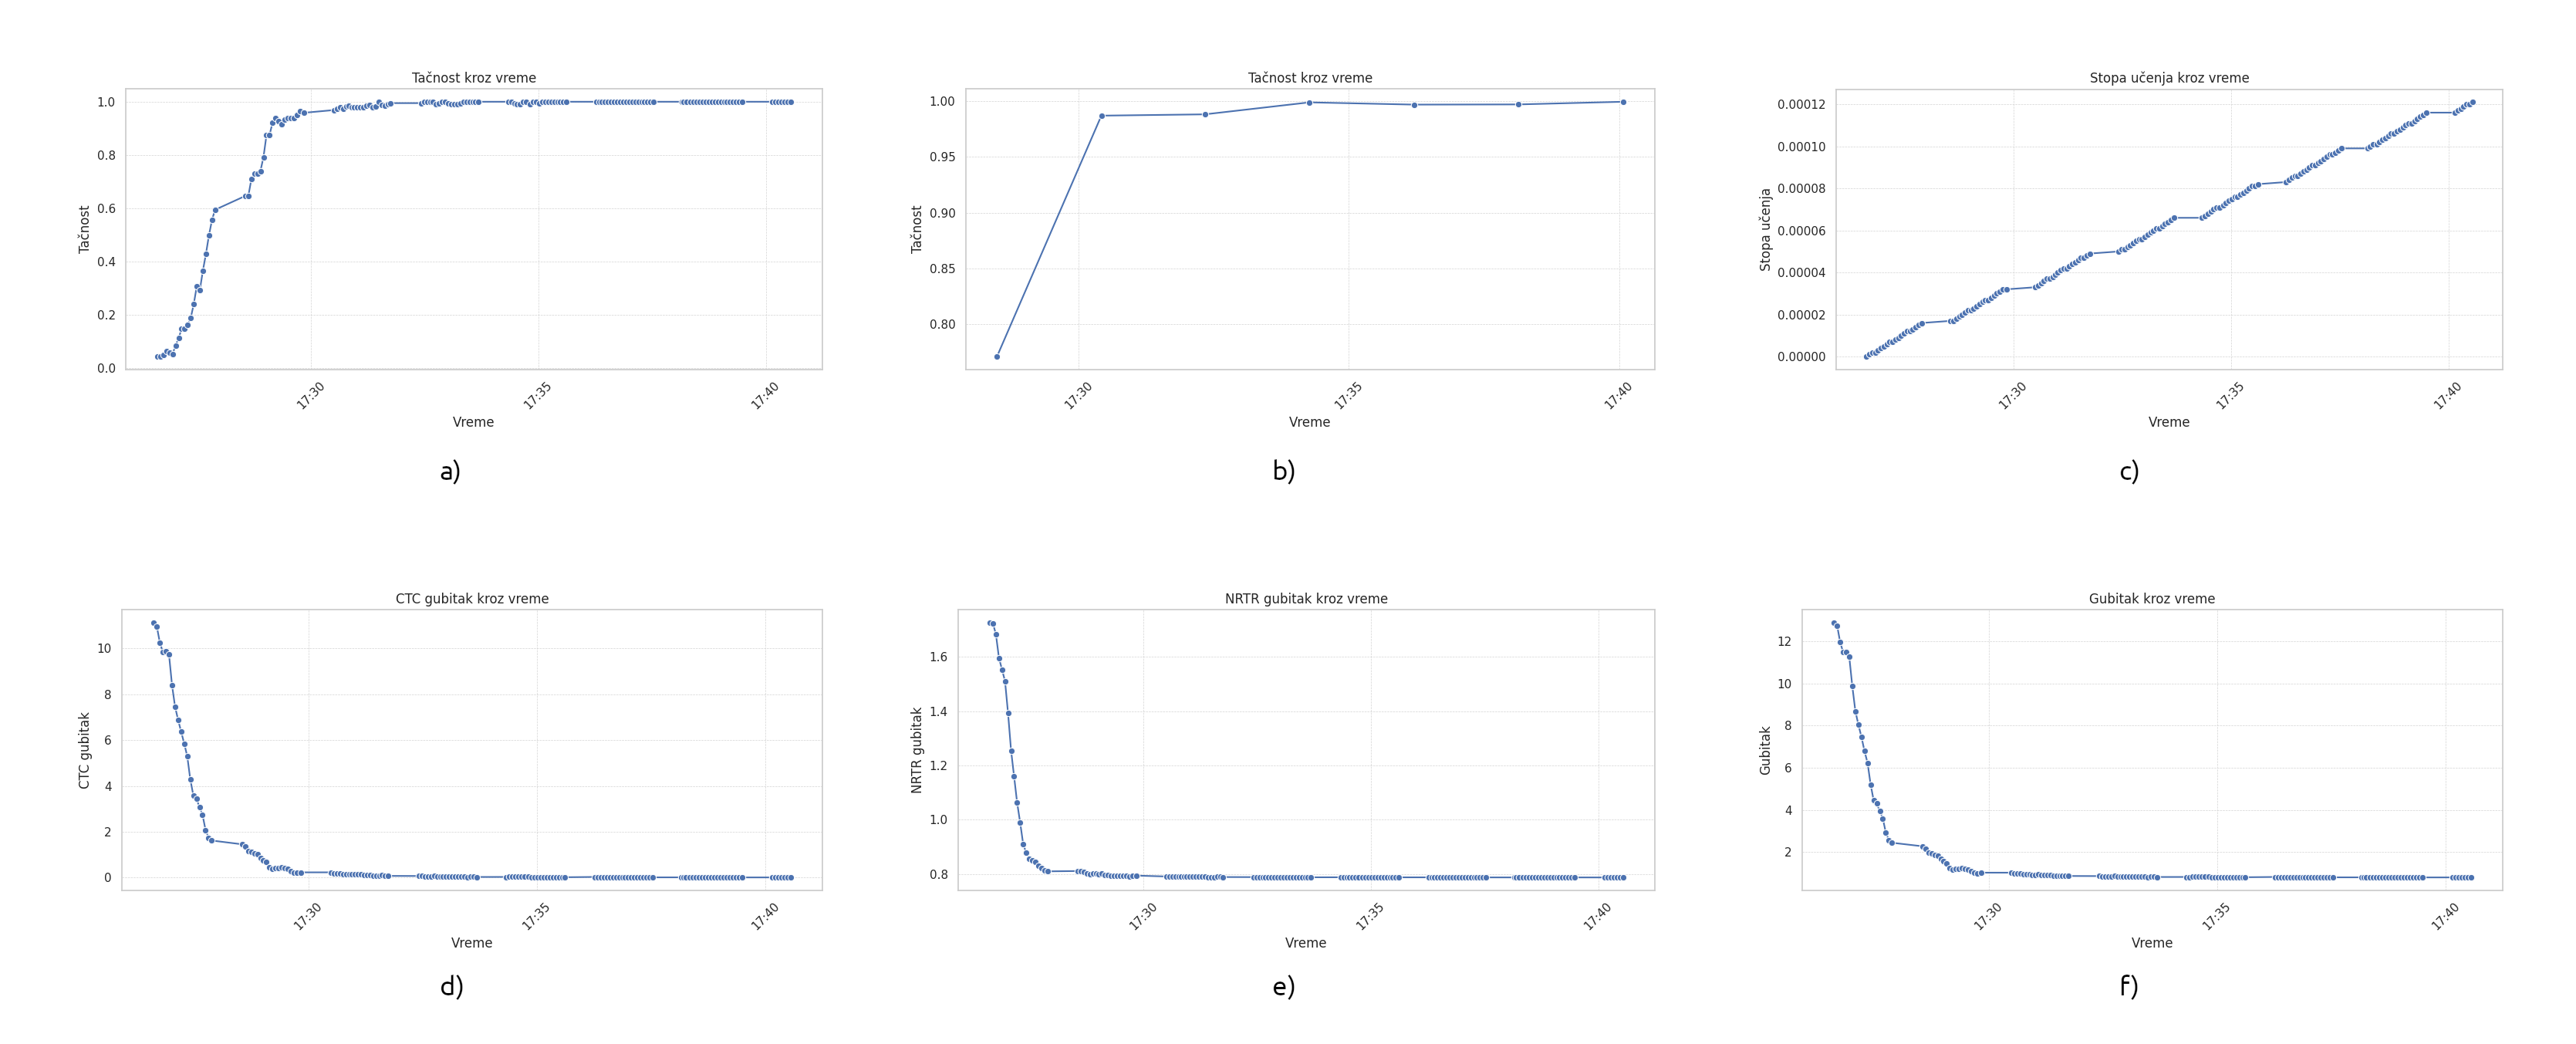
\includegraphics[width=\textwidth]{assets/synthetic-data-metrics.png}
		\caption{Metrike u toku treniranja modela sa sintetičkim podacima. a) Tačnost modela na trening podacima u toku obučavanja modela. b) Tačnost modela na validacionim podacima u toku obučavanja modela. c) Promena vrednosti stope učenja u toku obučavanja modela. d) CTC gubitak u toku obučavanja modela. e) NRTR gubitak u toku obučavanja modela f) Gubitak u toku obučavanja modela.}
		\label{fig:synthetic-data-metrics}
	\end{figure}
	
	Sintetički podaci su značajno povećali količinu i kontenstualnu raznovrsnost podataka. Iako sam sintetičkih podataka imao dosta više, trning je i ponovo trajao relativno kratko. Model je konvergirao za 10-ak minuta i dostigao tačnost od 100\% (Slika \ref{fig:synthetic-data-metrics}(a)) na trening skupu i najveću tačnost od 99.95\% (Slika \ref{fig:synthetic-data-metrics}(b)) na validacionom skupu dostigao za 15-ak minuta treniranja (Slika \ref{fig:train-code-synthetic-data}).\newline
	
	Skup sintetičkih podataka sam podelio u sledeće podskupove:
	\begin{itemize}
		\item Trening skup je činilo 70\% podataka, što je 83.300 slika
		\item Validacioni skup je činilo 15\% podataka, što je 17.850 slika
		\item Test skup je činilo 15\% podataka, što je 17.850 slika
	\end{itemize}
	
	\begin{figure}[H]
		\centering
		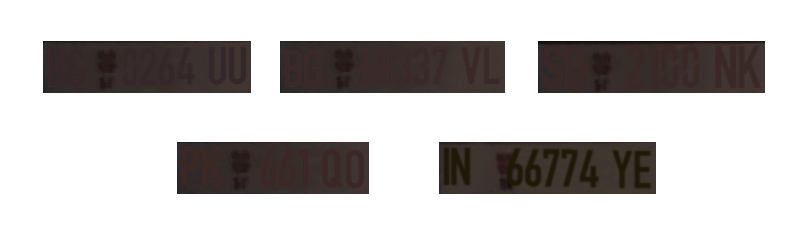
\includegraphics[width=\textwidth]{assets/bad-predictions-synthetic-data-model.png}
		\caption{Primeri slika tablica koje je model treniran samo sa sintetičkim podacima pogrešno prediktovao}
		\label{fig:bad-predictions-synthetic-data-model}
	\end{figure}
	
	Na nezavisnom testnom skupu podataka model je pogrešno prediktovao samo 5 od 17.850 slika, beležeći tačnost od 99.97\% na nezavisnom skupu podataka. Slike tablica koje nisu dobro prediktovane nalaze se na Slici \ref{fig:bad-predictions-synthetic-data-model}. Jasno se vidi da je zajednička karakteristika prve četiri slike to što se nalaze na tamnim pozadinama sa tekstom čija boja nije lako separabilna od boje pozadine. Poslednja prikazana slika tablice na Slici \ref{fig:bad-predictions-synthetic-data-model} ima veću razliku u boji između teksta i pozadine, a razlog zbog kojeg je bila neuspešna jeste grb sa tablice koji se našao direktno iza prve cifre, pa je model prvu cifru 6 prepozano kao \$.
	
	Ovaj model, u odnosu na model treniran na realnim slikama, ima manji ali i dalje visok stepen sigurnosti prilikom predikcije. Presečnna sigurnost modela treniranog na sintetičkom skupu podataka je 98,73\% na testnom sintetičkom skupu podataka.
	
	\subsubsection{Treniranje koristeći realne i sintetičke podatke}
	Finalni skup podataka koji sam koristio za treniranje modela predstavlja kombinaciju realnih i sintetičkih podataka. Idealno, za treniranje bih pretežno koristio realne podatke, a sintetičke podatke bih dodavao kako bih doprineo diverzifikaicji skupa realnih podataka. Na taj način se osiguravamo da kontekst koji model uči tokom treniranja što vernije odražava uslove u kojima će model funkcionisati u praksi. Međutim, uzevši u obzir da nisam imao pristup većem skupu realnih podataka od onog koji sam koristio, morao sam da nadoknadim taj nedostatak dodaanjem velikog broja sinetičkih podataka.
	
	\begin{figure}[H]
		\centering
		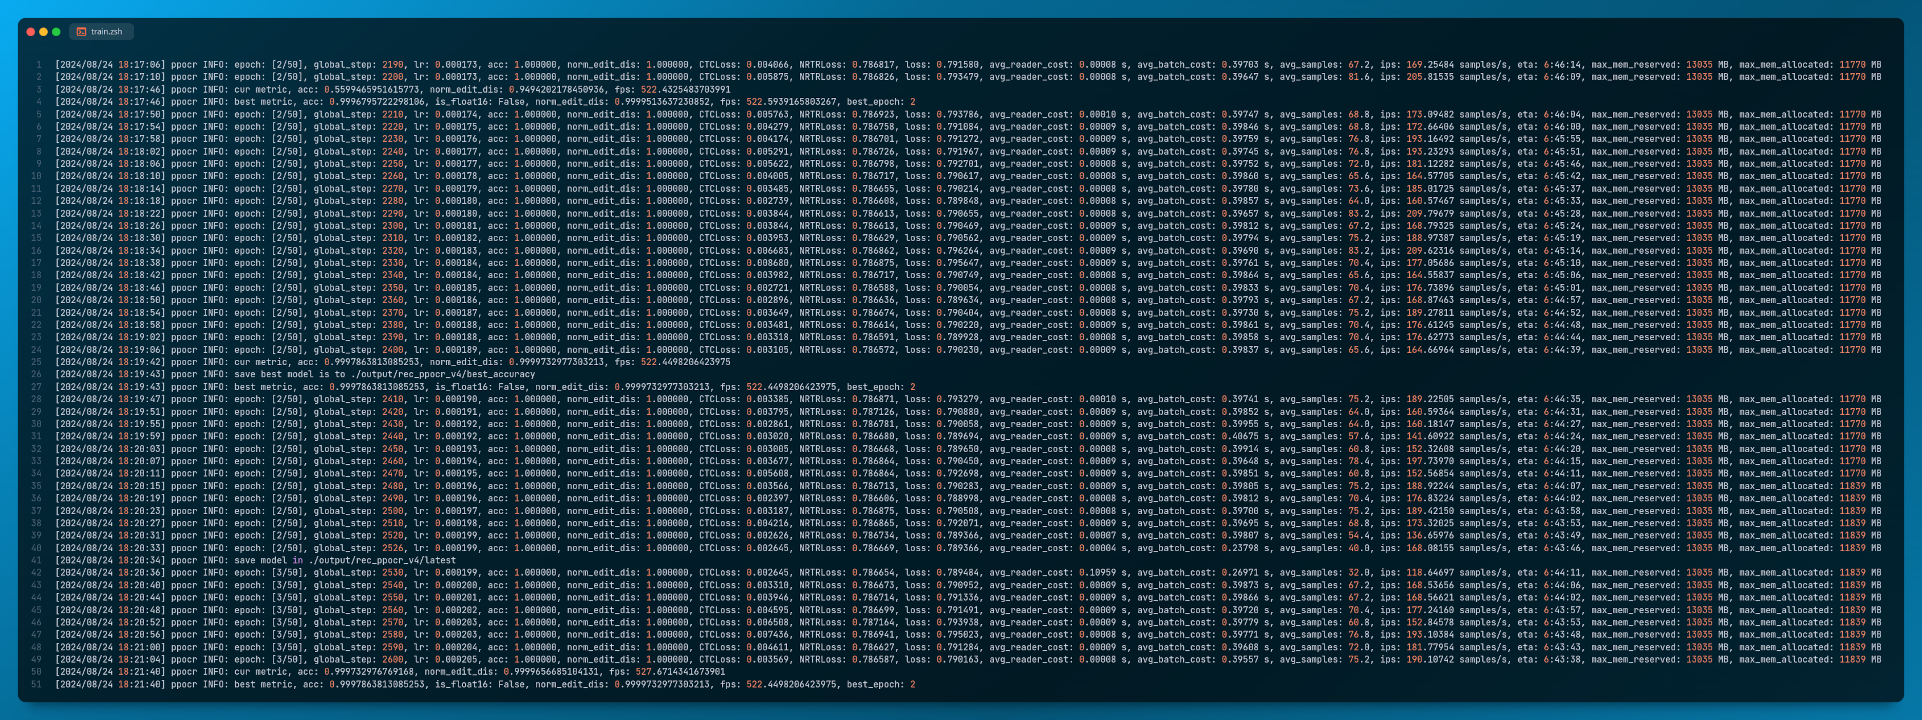
\includegraphics[width=\textwidth]{assets/train-code-real-and-synthetic-data.png}
		\caption{Krajnja faza procesa treniranja modela za detekciju teksta na spojenom skupu realnih i sintetičkih podataka}
		\label{fig:train-code-real-and-synthetic-data}
	\end{figure}

	\begin{figure}[H]
		\centering
		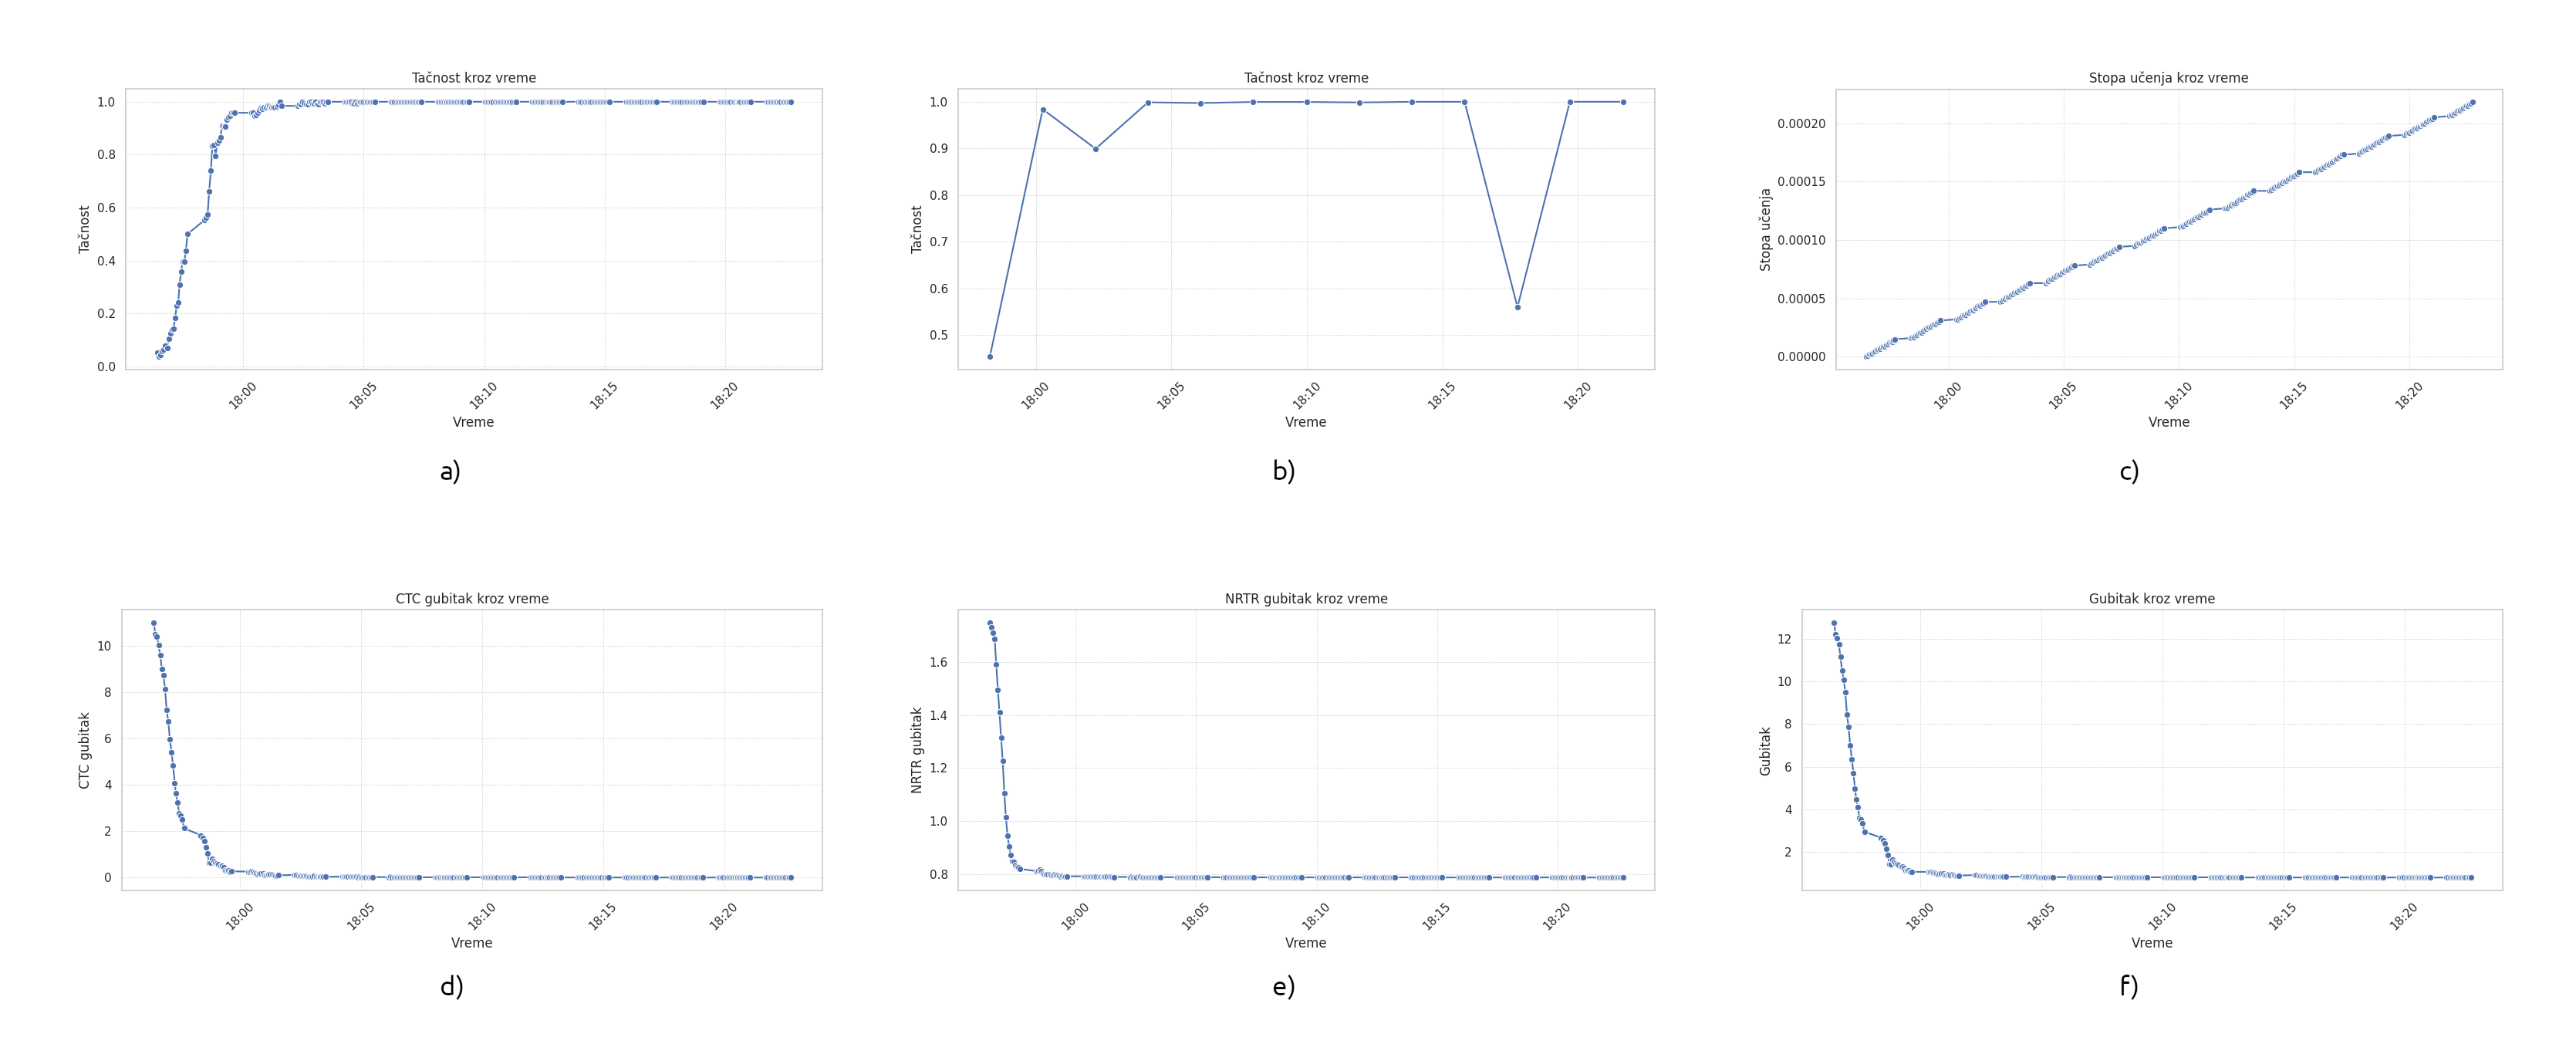
\includegraphics[width=\textwidth]{assets/real-and-synthetic-data-metrics.png}
		\caption{Metrike u toku treniranja modela sa realnim i sintetičkim podacima. a) Tačnost modela na trening podacima u toku obučavanja modela. b) Tačnost modela na validacionim podacima u toku obučavanja modela. c) Promena vrednosti stope učenja u toku obučavanja modela. d) CTC gubitak u toku obučavanja modela. e) NRTR gubitak u toku obučavanja modela f) Gubitak u toku obučavanja modela.}
		\label{fig:real-and-synthetic-data-metrics}
	\end{figure}
	
	Trening na spojenom skupu ralnih i sintetičkih podataka je trajao oko 30 minuta. Model je dostigao tačnost od 100\% (Slika \ref{fig:real-and-synthetic-data-metrics}(a)) na trening skupu i 99.97\% (Slika \ref{fig:real-and-synthetic-data-metrics}(b)) na validacionom skupu podataka (Slika \ref{fig:train-code-real-and-synthetic-data}).\newline
	
	Kombinovani skup realnih i sintetičkih podataka sam podelio u sledeće podskupove:
	\begin{itemize}
		\item Trening skup je činilo 70\% podataka, što je 87.386 slika, od kojih je 4.086 realnih i 83.300 sintetičkih slika
		\item Validacioni skup je činilo 15\% podataka, što je 18.725 slika, od kojih je 875 realnih i 17.850 sintetičkih slika
		\item Test skup je činilo 15\% podataka, što je 18.725 slika, od kojih je 875 realnih i 17.850 sintetičkih slika
	\end{itemize}
	
	\begin{figure}[H]
		\centering
		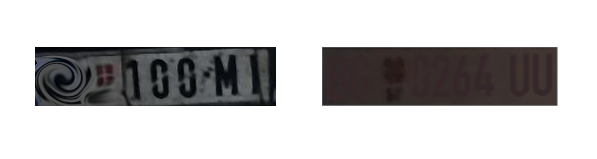
\includegraphics[width=\textwidth]{assets/bad-predictions-real-and-synthetic-data-model.png}
		\caption{Primeri slika tablica koje je model treniran na realnih i sintetičkim podacima pogrešno prediktovao}
		\label{fig:bad-predictions-real-and-synthetic-data-model}
	\end{figure}
	
	Na nezavisnom testnom skupu podataka model je pogrešno prediktovao samo 2 od 18.725 slika, beležeći tačnost od 99.98\% na nezavisnom skupu podataka. Slike tablica koje nisu dobro prediktovane nalaze se na Slici \ref{fig:bad-predictions-real-and-synthetic-data-model}. Model koji je treniran na kombinovanom skupu realnih i sintetičkih podataka je imao problem sa predikcijom na slici tablice koja je pomoćnim trakama koje prelaze preko teksta zakačena za automobil. Ovaj primer ilustruje korišćenje softvera u realnim uslovima, gde osoba koja kreira sintetički skup podataka ne može uvek da predvidi sve moguće scenarije koji se mogu desiti u praksi. To dodatno naglašava važnost pravih podataka i objašnjava zašto svi koji razvijaju ozbiljne modele teže ka potrazi za pravim podacima. Ovaj model, kako i model treniran samo na sintetičkim podacima takođe pokazuje porblem sa izrarito malim razlikama u boji između teksta i pozadine, ali u manjoj meri. Takvo pogrešno prepoznavanje teksta može se smatrati prihvatljivim, s obzirom na to da je veoma teško pročitati šta zaprao piše na takvoj slici.
	
	Kombinovanjem realnih i sintetičkih podataka za vreme treninga, stepen sigurnosti modela prilikom predikcije je povećan u odnosu na model treniran samo nad sintetičkim podacima. Presečnna sigurnost modela je 99,32\% na testnom skupu podataka. Sigurnost je i dalje nešto manja u odnosu na model treniran koristeći isključivo realne podatke, što ukazuje na važnost korišćenja realnih podataka prilikom treniranja modela.
	
	\subsubsection{Uporedna analiza tačnosti modela na sva tri testna seta}
	
	\begin{table}[H]
		\centering
		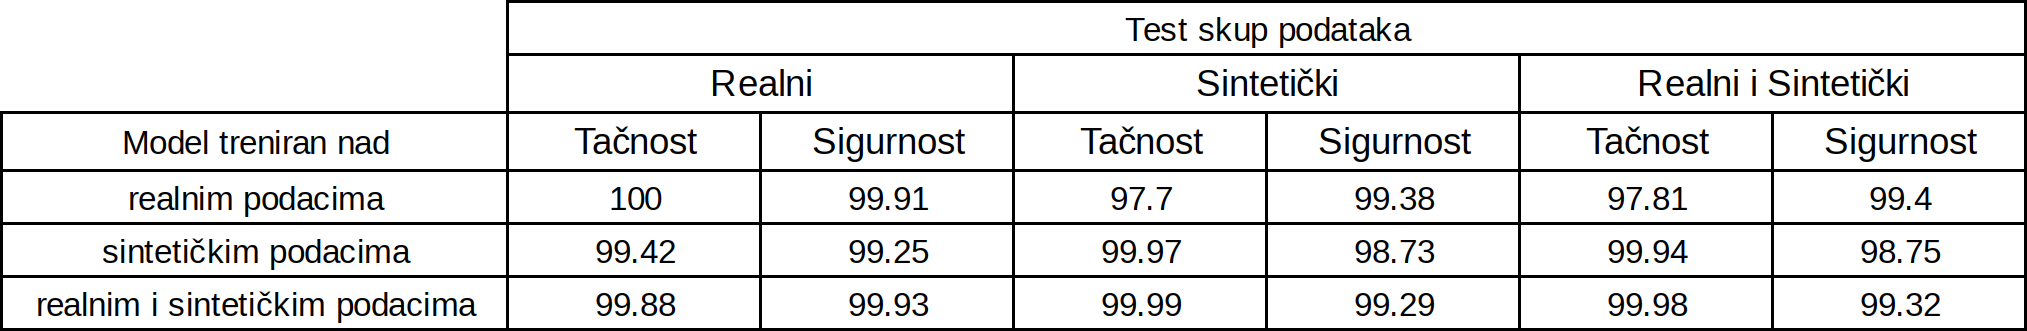
\includegraphics[width=\textwidth]{assets/comparative-analysis-on-test-set.png}
		\caption{Uploredna analiza tačnosti tri obučena modela na zasebnim testnim skupovima}
		\label{fig:comparative-analysis-on-test-set}
	\end{table}

	Nakon treniranja tri modela na opisanim skupovima podataka, uporedio sam njihovu tačnost i sigurnost prilikom predikcije na svim testnim skupovima (Tabela \ref{fig:comparative-analysis-on-test-set}).
	
	Model koji je treniran i testiran na realnim podacima postigao je najveću tačnost i sigurnost, što je očekivano s obzirom na to da su trening i testni skup sadržavali vrlo malo slika tablica izdatih isključivo na teritoriji Beograda. Ipak, iako ovaj model ima najbolju tačnost na realnim testnim podacima, njegova tačnost na ostalim testnim skupovima je značajno lošija u odnosu na ostale modele. Zbog toga, model koji je treniran samo na realnim podacima nije najbolji izbor među tri ponuđena modela.
	
	Najlošiju tačnost i sigurnost imao je model treniran na realnim, a testiran na sintetičkim podacima. Vrlo sličan, ali nešto bolji rezultat ostvario je isti model na testnom skupu kombinovanih realnih i sintetičkih podataka. Razlog za ovo je što je model tokom treninga na prvim dvema pozicijama video samo \enquote{BG} niz karaktera, dok su testni skupovi sadržali tablice iz svih opština Srbije koje imaju pravo da izdaju registarske tablice. Dodatno, korišćeni font za generisanje sintetičkih podataka je ručno napravljen i možda nije idealno replicirao originalni font, što je moglo uticati na tačnost.
	
	Iako nema apsolutno najveću tačnost i sigurnost, najbolji model za korišćenje u realnim uslovima je onaj treniran na realnim i sintetičkim podacima. Razlika u odnosu na model sa najvećom tačnošću je samo 0,02\%, što se može smatrati zanemarljivom. Ovaj model je imao najraznovrsniji i najobimniji trening skup, što mu uz odlične rezultate na validacionim i testnim skupovima daje prednost u izboru.
	\newpage
	
	\section{Buduća poboljšanja}
	
	\subsection{Dodatna diverzifikacija skupa podataka}
	Iako model koji sam trenirao pokazuje odlične performanse prepoznavanja teksta sa tablica automobila izdatih na teritoriji Republike Srbije, nije očekivano da će idealno raditi na tablicama vozila iz drugih država zbog razlika u dizajnu, fontovima i karakterima. Svaka zemlja ima svoje specifične standarde kada je reč o izgledu registarskih tablica, što uključuje različite boje, oblike i stilove fonta. Na primer, tablice iz nekih drugih zemalja mogu koristiti karaktere koji se razlikuju od onih na srpskim tablicama, što može dovesti do problema u prepoznavanju.
	
	\begin{figure}[H]
		\centering
		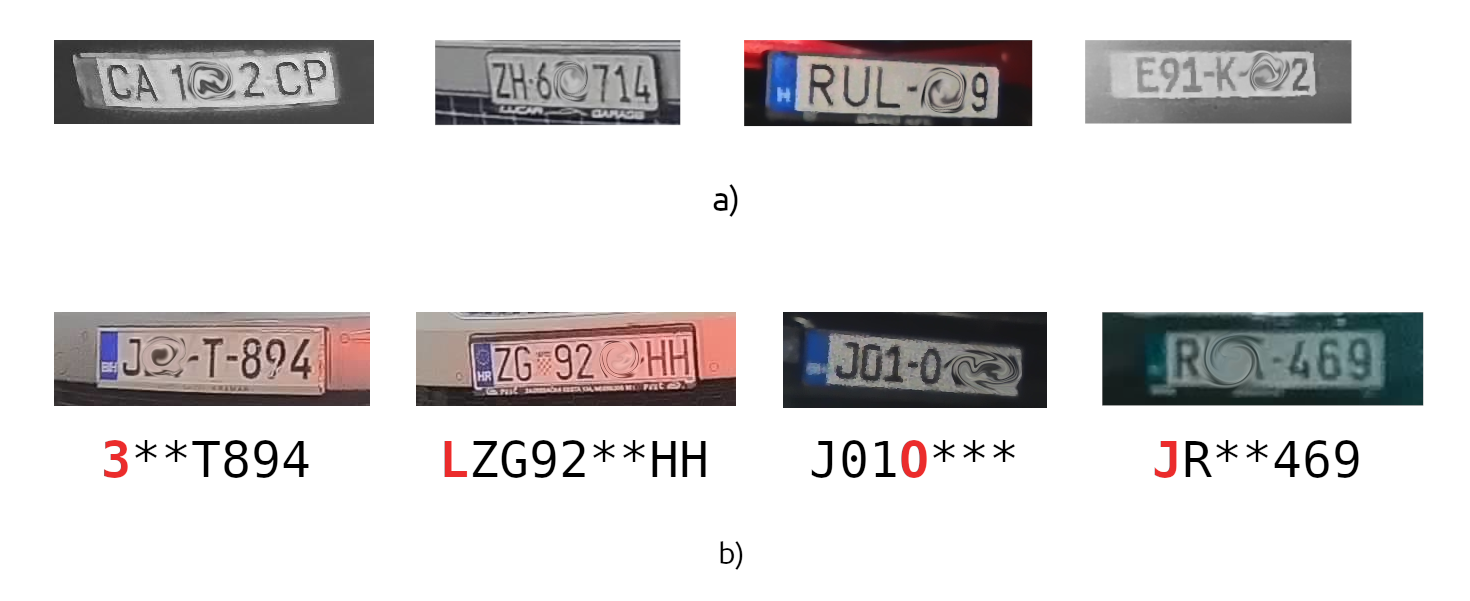
\includegraphics[width=\textwidth]{assets/good-and-bad-predictions.png}
		\caption{Primeri slika stranih tablica. a) Primeri dobro prepoznatog teksta sa slika stranih tablica. b) Primeri loše prepoznatog teksta sa slika stranih tablica sa naznačenim greškama prilikom predikcije.}
		\label{fig:good-and-bad-predictions}
	\end{figure}
	
	Bez obzira na to što model prilično dobro prepoznaje tekst sa tablica iz država koje nije video, bilo bi korisno dodati takve podatke u trening skup. Različite države često imaju specifične fontove ili karaktere koje model nije imao priliku da vidi tokom treniranja sa srpskim tablicama. To može dovesti do grešaka, posebno kada se radi o sličnim karakterima, kao što su \enquote{O} i \enquote{0} (Slika \ref{fig:good-and-bad-predictions} (b)) ili \enquote{I} i \enquote{1}. U takvim slučajevima, model može lako napraviti pogrešna prepoznavanja, što može uticati na ukupnu tačnost i pouzdanost.
	
	Zbog ovih razlika, važno je obogatiti trening skup dodatnim podacima iz različitih zemalja kako bi model poboljšao performanse na stranim tablicama. Uključivanje raznovrsnih podataka može pomoći u smanjenju grešaka i povećanju preciznosti prepoznavanja, čime bi se postigla veća efikasnost u stvarnim uslovima.
	
	\subsection{Prepoznavanje teksta na više tablica sa iste slike}
	
	Trenutna verzija sistema za automatsko prepoznavanje teksta sa tablica automobila podržava pronalaženje i prepoznavanje teksta sa tačno jedne, najveće, tablice sa slike. Ovakvo ponašanje sistema nije idealno u slučajevima kada želimo da sa jedne slike dobijemo informacije o svim registarskim tablicama. Primer takvog sistema bi bio sistem za nadzor parking zona koji se može koristiti za automatsku naplatu parkinga ukoliko korisnik poveže svoj parking nalog sa konkretnim tablicama, ili za pronalaženje lokacije parkiranog automobila.
	
	Verzija sistema koja bi radila prepoznavanje teksta sa svih tablica na slici treba da vrati niz rezultata prepoznavanja teksta, gde bi svaki element niza pored slike isečka tablice i prepoznatog teksta imao i informaciju o tačnoj poziciji tablice na slici. Tačna pozicija tablice bi bila korisna za detekciju tačnog mesta na kojem se korisnik parkirao.
	
	\subsection{Ubrzanje rada sistema}
	
	Trenutna verzija sistema za automatsko prepoznavanje teksta sa tablica automobila obrađuje jednu ulaznu sliku u proseku oko 1000ms. Iako trenutno vreme izvršavanja nije previše dugo, kako bi sistem bio performantniji i bio u stanju da prihvati više upita potrebno je skratiti vreme izvršavanja izbacivanjem komponenti koje nisu neophodne za rad.
	
	Jedan od koraka ka ubrzanju sistema jeste uklanjanje modela za detekciju teksta. Trenutno, model za detekciju teksta ima ulogu da nakon detekcije tablica sa slike finije pronađe regiju u kojoj se nalazi samo tekst od interesa prilikom obrade tablice. Taj korak bi mogao biti izbegnut kada bi odradili dodatno dotreniravanje modela za detekciju tablica tako da model za detekciju tablica inicijalno vraća regiju relativno usko oko teksta od interesa bez teksta koji se može naći na okvirima tablica. Pored toga, korišćenje modela za segmentaciju instance umesto detekcije objekta dovodi do znatno efikasnije detekcije regije koju zauzima samo registarska tablica, bez okvira i pozadine koji se mogu obuhvatiti pravougaonom detekcijom objekta.
	
	Drugi korak bi bio korišćenje manjeg inicijalnog modela umesto modela predviđenog da radi na serveru. U tom slučaju performanse u preciznosti prepoznavanja teksta sa tablica automobila bi opale u nekoj meri, ali bi pad preciznosti bio veoma mali i merljiv tek nad značajno velikim skupom podataka. S druge strane, ubrzanje rada modela bi bilo značajno.
	\newpage
	
	\section{Zaključak}
	
	\subsection{Važnost treniranja modela sa podacima sličnim onima koji će biti korišćeni}
	Treniranje modela sa podacima koji su slični onima koji će se koristiti u stvarnim uslovima je neophodno za postizanje visoke tačnosti modela. Kada se model trenira na relevantnim i reprezentativnim podacima, bolje može da prepozna obrasce i karakteristike koje će se pojaviti u novim, nepoznatim podacima.
	
	Ako su podaci korišćeni za treniranje značajno različiti od onih koji se koriste u praksi, model može imati problem sa generalizacijom, što može dovesti do loših predikcija. Stoga je važno osigurati da skup podataka za treniranje obuhvata raznovrsne i realistične primere koji odražavaju stvarne uslove rada.
	
	Model opšte namene za prepoznavanje teksta, koji sam koristio kao startni model za treniranje na slikama tablica, ima neprihvatljivo lošu tačnost za produkcione uslove. Tačnost startnog modela na realnim podacima je 87.68\%, na sintetičkim 88.38\% i na kombinovanim skupu ralnih i sintetičkih podataka 88.35\%. Primetno je da se startni model prilikom evaluacije konzistentno ponaša na sva tri skupa podataka sa kojima sam trenirao model, što je dodatni pokazatelj da prilikom treniranja modela za prepoznavanje teksta na tablicama nije došlo do prekomerne prilagođenosti podacima, već je startni model naučio da prepoznaje novi tip podataka.
	\newpage
	
	\printbibliography
	\addcontentsline{toc}{section}{Literatura}
\end{document}